\documentclass{mcmthesis}

\mcmsetup{CTeX = true,   % 使用 CTeX 套装时,设置为 true
        tcn = 2215432, problem = E,
        sheet = true, titleinsheet = true, keywordsinsheet = true,
        titlepage = false, abstract = false}
\geometry{left=0.75in,right=0.75in,top=1in,bottom=1in}
\numberwithin{figure}{section}
\numberwithin{table}{section}
\numberwithin{equation}{section}
\usepackage{newtxtext}
\usepackage{lipsum}
\usepackage{palatino}
\usepackage{hyperref}
\usepackage{booktabs}
\usepackage{subfigure}
\usepackage{graphicx}
\usepackage{pythonhighlight}
\usepackage{indentfirst}%首段自动缩进
\usepackage{colortbl}
\usepackage{apacite}
\usepackage{natbib}
\usepackage{tablefootnote}
\usepackage{multicol}
%算法四部曲↓
\usepackage{algorithm}
\usepackage{algpseudocode}
\usepackage{amsmath}
\usepackage{algorithmicx}
% \usepackage{threeparttable}
\definecolor{lightBlue}{rgb}{0.867,0.922, 0.969}
\setlength{\parindent}{2em}
\title{123}
\setlength{\headheight}{15pt}

\begin{document}
\renewcommand{\algorithmicrequire}{\textbf{Input:}}  % Use Input in the format of Algorithm
\renewcommand{\algorithmicensure}{\textbf{Output:}} % Use Output in the format of Algorithm
\begin{abstract}



\begin{keywords}
\end{keywords}
\end{abstract}
\maketitle

\tableofcontents
  \thispagestyle{empty}
  \newpage
  \setcounter{page}{1}
%%
%%Generate the Memorandum, if it's needed.
%\memoto{\LaTeX{}studio}
%\memofrom{Liam Huang}
%\memosubject{Happy \TeX{}ing!}
%\memodate{\today}
%%\logo{\LARGE I'm pretending to be a LOGO!}
%\begin{memo}[Memorandum]
%  \lipsum[1-3]
%\end{memo}

\section{Introduction}

\subsection{Problem Restatement}
Considering that the carbon dioxide can be sequestered in both forests 
and wooden products, it's reasonable that more carbon will be stored by forests with the 
appropriate combination of the regrowth of younger forests and the wooden products.
Thus, forest managers are ought to deliberate about the balance between the value of forests 
as living tress to grow and absorb the carbon and the value of forests harvested as wooden products.
What's more, the forest managers should not only consider the factors about forests such as 
type and age of forests, geography, topography, and benefits and lifespan of forest products,
but also the conservation and diversity of wild species, recreational uses and cultural considerations.
\begin{enumerate}
    \item [1.] Design a carbon sequestration model to calculate the amount of carbon dioxide 
    sequestered by a forest and its products, which also determines what kind of manage plan is
    most efficient at sequestering carbon.
    \item [2.] Develop a decision model consisting of various ways that forests are valued (including
    carbon sequestration) for forest managers to understand the best use of a forest. Consider 
    the following questions. What is the scope of the management plan that your decision model might suggest?
    Are there any conditions that the forests should not be harvested?
    Whether there is a transition point between management plans applicable to all forests?
    How can the characteristics of a particular forest and its location be used 
    to determine transition points between management plans?
    \item [3.] Apply your models to various forests. Identify a forest that your decision model 
    would suggest the inclusion of harvesting in its management plan.
    How much carbon dioxide can be sequestered by this forest and its products in 100 years?
    What kind of forest management plan should be carried out for this forest? Why it's best?
    The best management plan is assumed to include a harvest interval of 10 
    years longer than current forest practices discussing strategies for transitioning 
    from existing to new schedules in a manner sensitive to the needs of forest managers 
    and all those who use forests.

    \item [4.] Some people think that we should never cut down any trees, but you've
    determined the forest which includes harvest in its management. Write a one-to-two-page
    non-technical newspaper articles to explain why your analysis including in the 
    management of the forest logging, rather than it remaining the same. Finally, your ariticle 
    should convince local community that it's the best decision for their forest.
\end{enumerate}

\subsection{Overview of Our Work}




\section{Assumptions and Justifications}
These are necessary assumptions for simplifying the model.
\begin{enumerate}
  \item [1.] 
\end{enumerate}

\newpage

\section{Notations}

\renewcommand\arraystretch{1.5}

\begin{table}[htpb!]
  \centering
  \caption{Notation Descriptions}
  \begin{tabular}{m{2.5cm}<{\centering}|m{12.5cm}<{\centering}}
  \toprule[1.5pt]
  \textbf{Symbol} & \textbf{Definition} \\ \hline
  $ \rm{DBH} $ & Diameter at Breast Height \\
  $ \beta_b $ & Conversion factor of coniferous trees\\
  $\beta_c$ & Conversion factor of broad leaf trees\\
  $ n $ & Total iteration years\\
  $ \lambda $ & Harvest rate\\
  $ M $ & Sequestered carbon mass in wooden products \\
  $ \rm{CarbonMass_f} $ & Sequestered carbon mass in forests \\
  $ \phi $ & Proportion in total product\\
  $ s $ & Scrap rate\\
  $ m $ & Decomposition rate \\
  $ K $ & Carrying Capacity \\
  $ N $ & Species population \\
  $ r $ & Population Growth Rate\\
  $ \alpha,\beta $ & Coefficient of Competition\\
  $ p $ & Rotation Years \\
  

  \bottomrule[1.5pt]
  \end{tabular}
\end{table}

\newpage

% 标题可能需要修改
\section{Model I}
\subsection{Cellular Automata based Population Size Prediction}

Cellular automata (CA) is a kind of grid dynamics model with discrete time, 
space and state, and local spatial interaction and temporal causality, which 
has the ability to simulate the space-time evolution process of complex system.
\par
Unlike general dynamical models, cellular automata are not determined by strictly 
defined physical equations or functions, but are composed of rules constructed by 
a series of models. Any model that satisfies these rules can be regarded as a cellular 
automata model. Therefore, cellular automata is a general term for a class of models, 
or a method framework. Its characteristic is that time, space and state are discrete, 
each variable only takes a finite number of states, and its state change rules are local 
in time and space.
\begin{figure}[htbp]
  \centering
  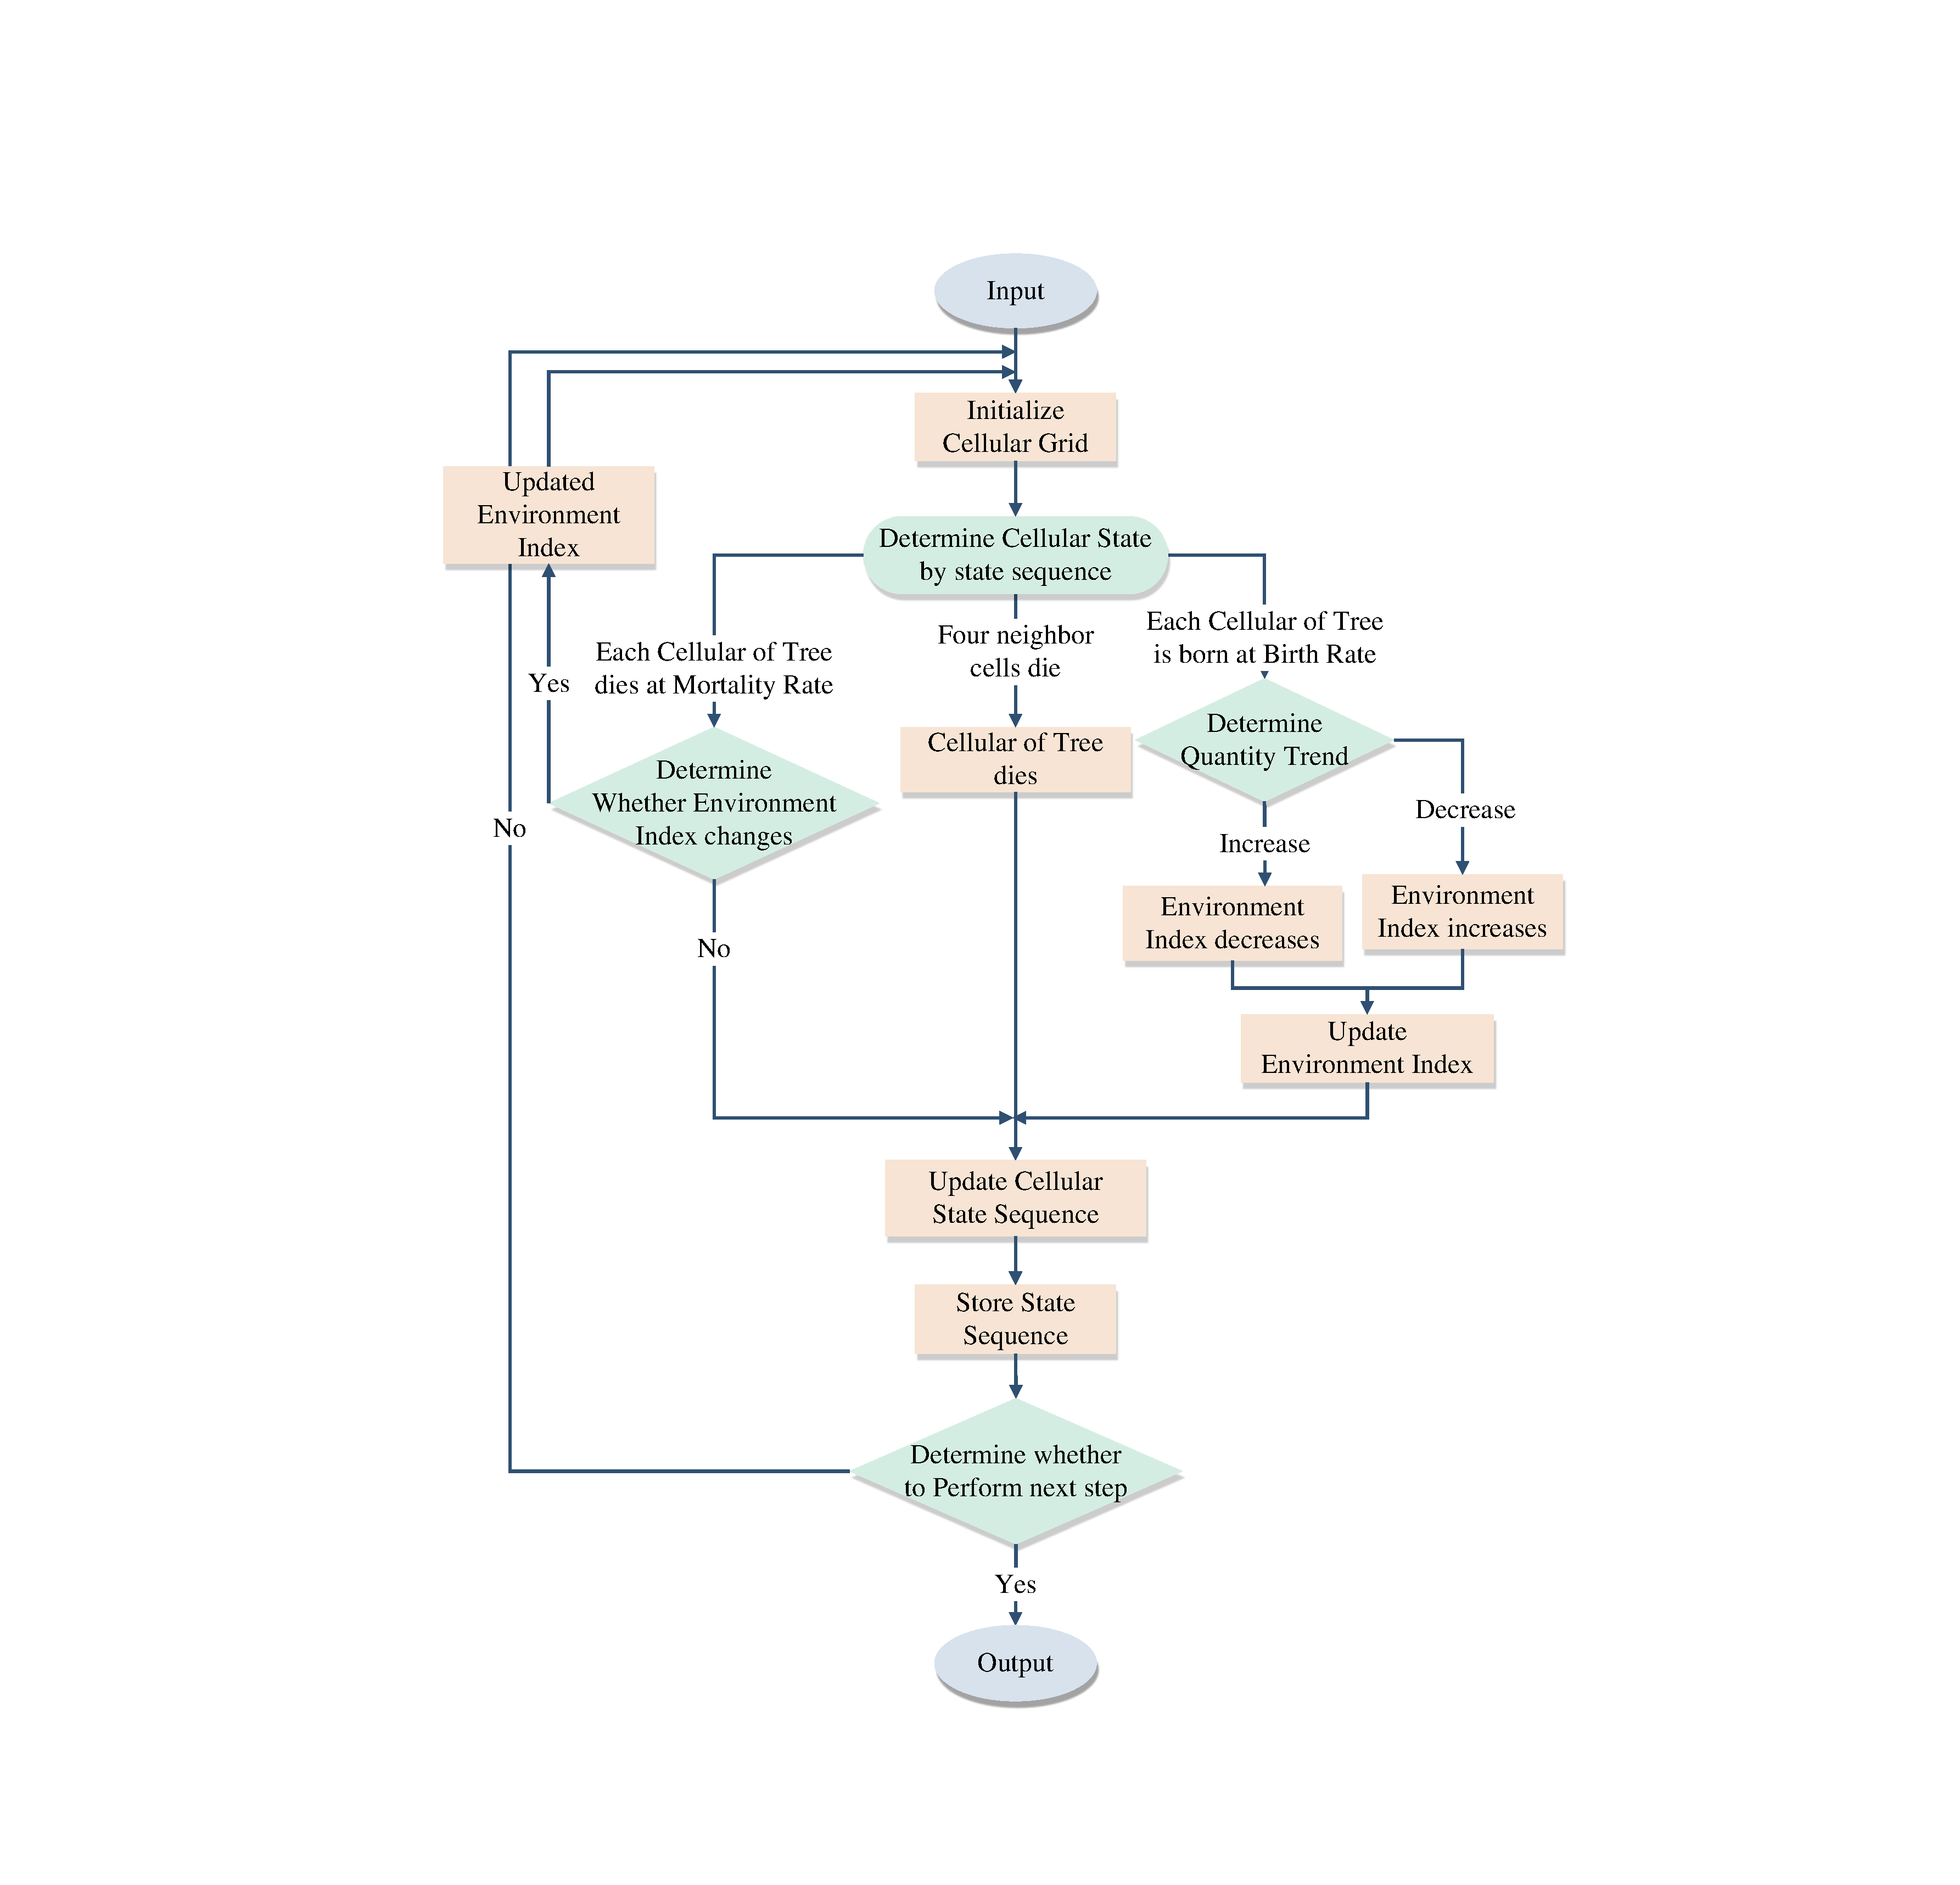
\includegraphics[width = 12cm]{code&pic/元胞自动机流程图.pdf}
  \caption{Block Diagram of typical Cellular Automata}\label{CA_Fig}
\end{figure}

The block diagram of a typical cellular automata is shown in Figure \ref{CA_Fig}, 
and the simulation result is shown in Figure \ref{CA_Result}, in which
we learn that the under the natural circumstances, the forestry population size
will reach and remain around 2100 per hectare. 

\begin{figure}[t]
  \centering
  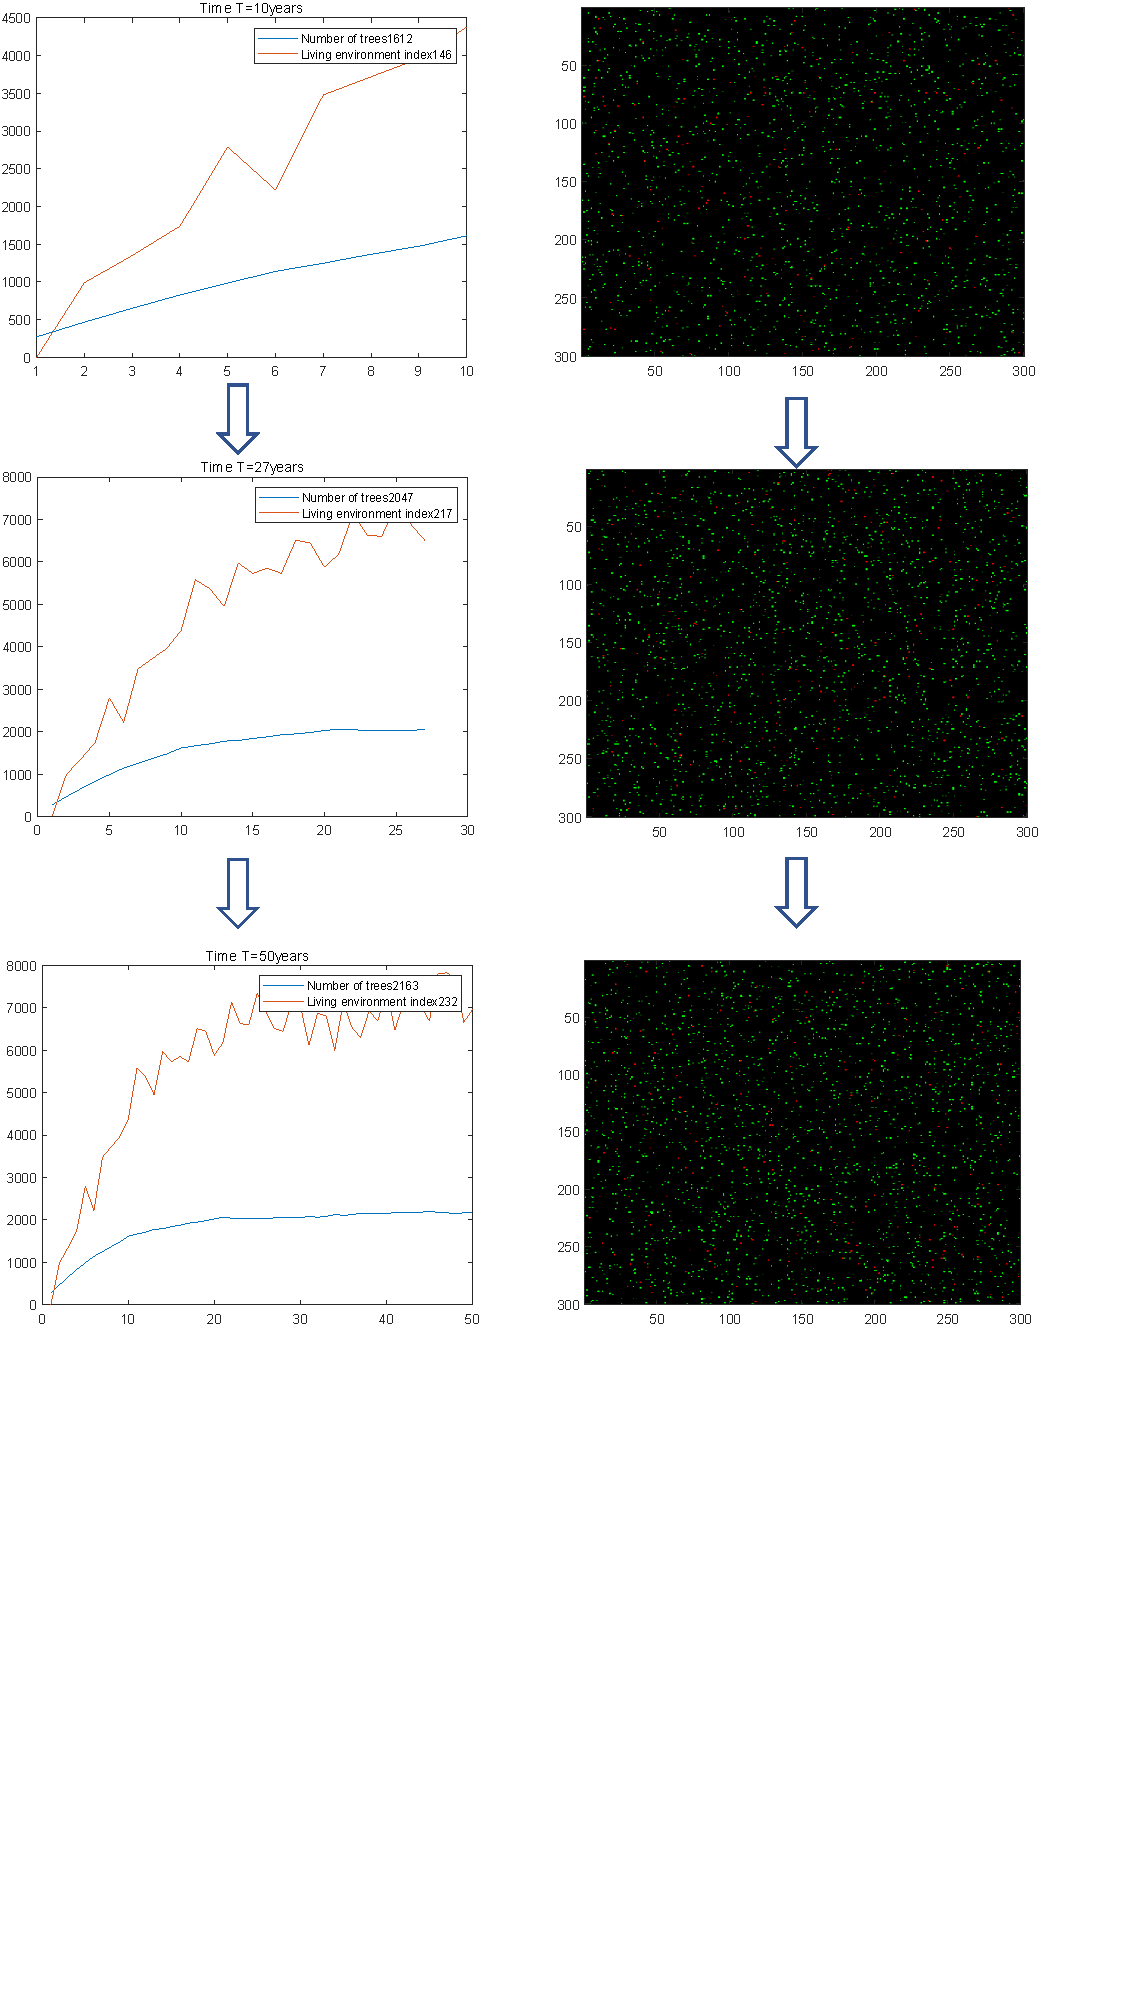
\includegraphics[width = 14cm]{code&pic/CA-pic.pdf}
  \caption{Result of Cellular Automation}\label{CA_Result}
\end{figure}

\subsection{Binary Timber Volume and Logistic based Carbon Sequestration Model}

In order to clearly demonstrate the amount of carbon sequestered by forests and their
products, we decide to consider the trunk volume of living trees as an estimation of 
total Volume of trees that are able to store carbon \citep{WangYan}. 
\par
For the living trees, we apply Binary Timber Volume Regression model \citep{LuoQingbang} 
to depict their growth as shown in Algorithm \ref{Binary Volume Algo}. 
It is significant
to point out that $ \beta_b $ and $ \beta_c $ are two \textbf{Conversion Factors} from
Timber Volume to Carbon Mass sequestered. Besides, the mass of carbon sequestered in
soil and leaves can be deemed as a constant which merely depends on the area
of coniferous and broad-leaved forests \citep{YanDeren2011}. 
\par
As for the wooden products, we consider $ w $ kinds of wooden products, each kind,
which decomposes at the rate of $ m_i (i = 1,\cdots, w) $, accounts for $ \phi_i$ 
of the total product mass \citep{2006Forest}. Note that the \textbf{harvest rate} $ \lambda $ and the product
proportion $ \phi $ are flexible regarding the circumstances, which are also 
the core of our forest management. And the harvest will be conducted every 
$ p $ years, which is \textbf{Rotation}. 
\par
What's more, we hold the view that 
the volume of wooden products derive from the volume of harvested trees with a certain
\textbf{Scrap Rate} $ s $. Suppose the harvested wood is stored in a well-organized
warehouse and the storage will become products in next $ p $ years, which means 
 $ \frac{1}{p} $ of all the storage will become products every year.
The complete idea is shown in Algorithm \ref{Product Algo}.
\par
\begin{figure}[ht]
  \begin{minipage}[htbp]{0.42\linewidth}
    The Scrap Rate is determined as following descriptions, which is also shown 
    in Figure \ref{RoundWood} on the right. There are two 
    manufacturing methods of Round Wood harvested from the forests. 
    \par
    One way is to trim the wood neatly into slabs in different shapes so that they can
    occupy most of the volume of the wood, which will be processed into softwood plywood, 
    panels and board. Meanwhile, the scrap will be manufactured into miscellaneous 
    products. It can approach the utilization rate of 81.3\%.
    \par
    The other kind of craft is to separate the bark and turn it into paper, and 
    the separated log can be processed into softwood and hardwood. The utilization 
    rate of this craft is able to reach almost 100\%.
  \end{minipage}
  \hfill
  \begin{minipage}[htbp]{0.5\linewidth}
    \begin{flushright}
      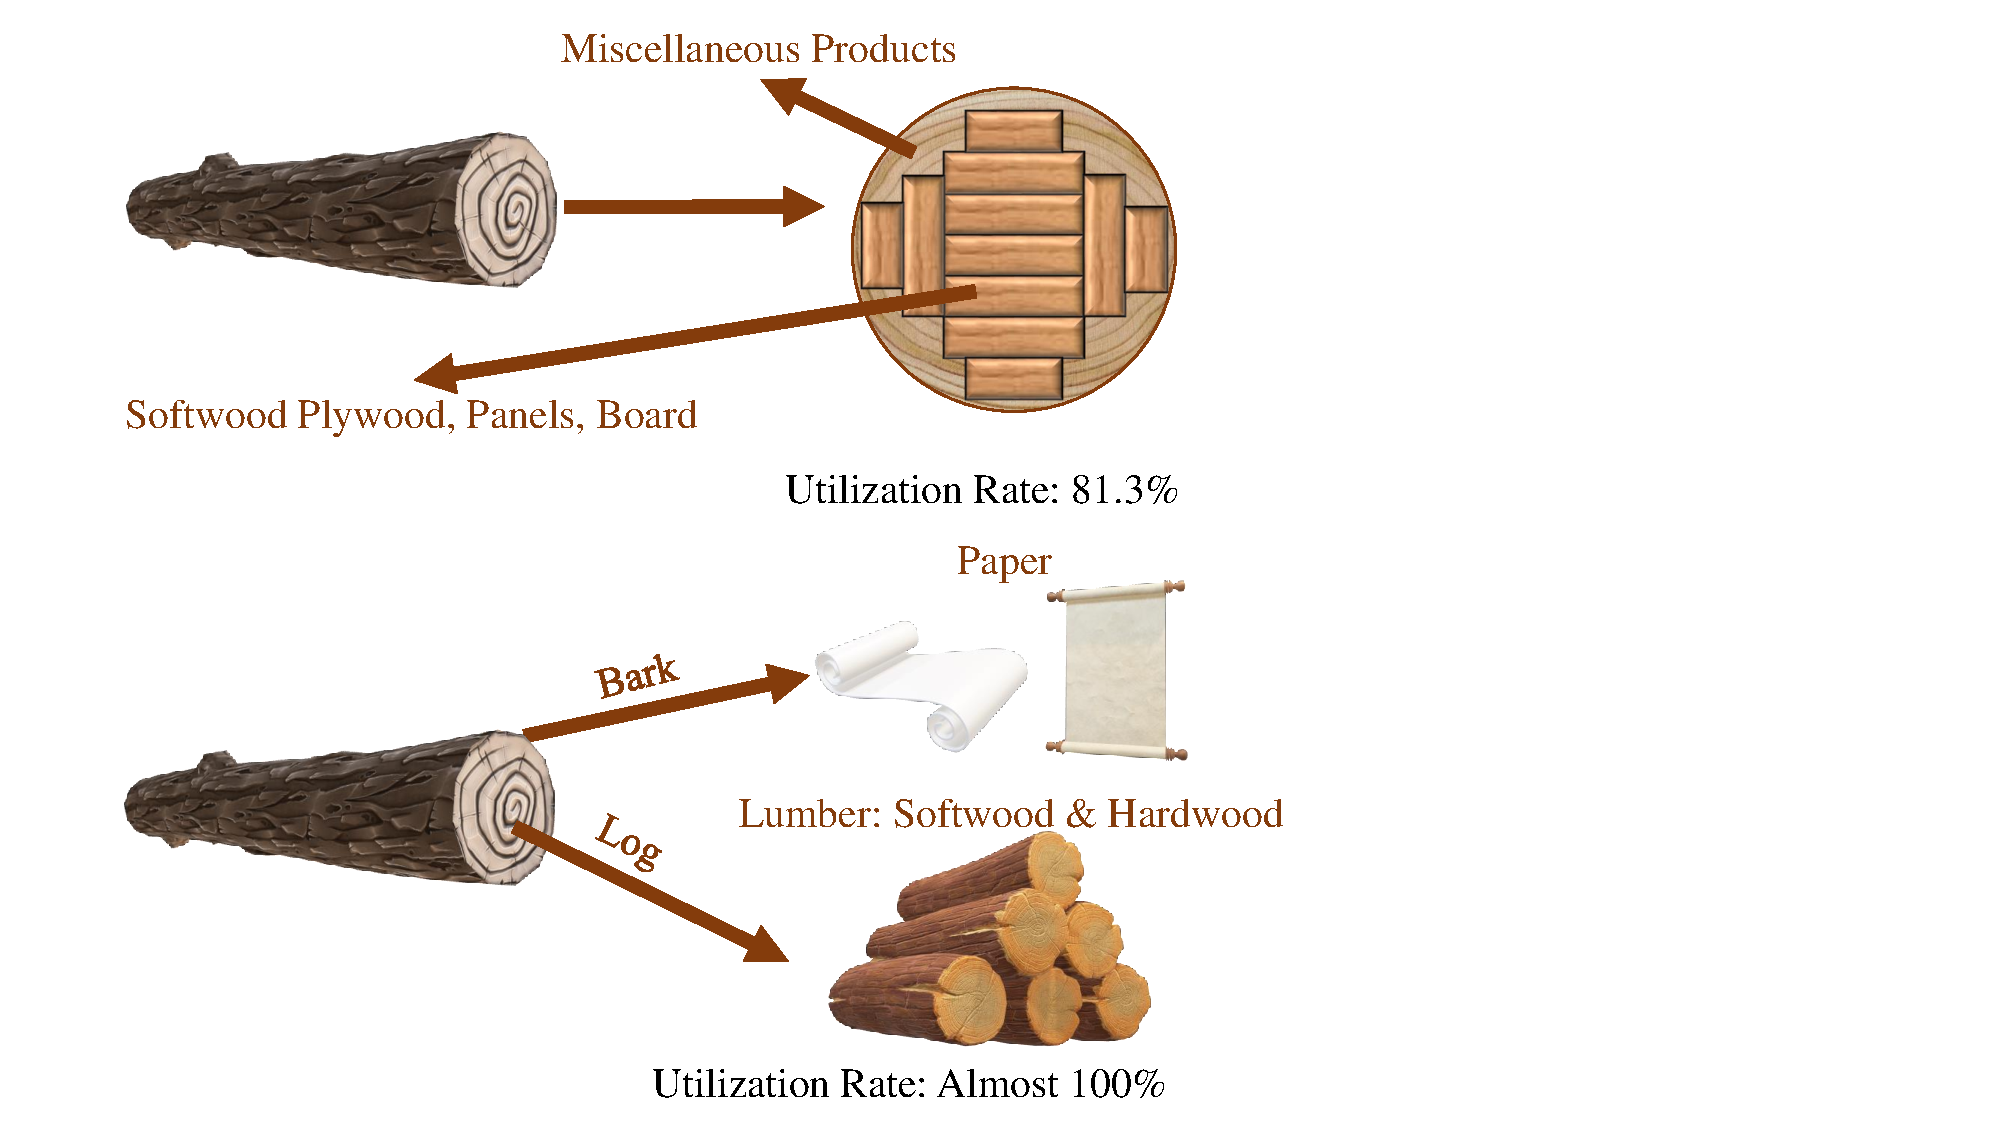
\includegraphics[width = 8.61cm]{code&pic/Roundwood cutting ways.pdf}
      \caption{Utilization Rate of Round Wood}\label{RoundWood}
    \end{flushright}
  \end{minipage}
\end{figure}




\begin{algorithm}[htbp]
    \caption{Binary Timber Volume Regression of Carbon Prediction Algorithm}\label{Binary Volume Algo}
    \begin{algorithmic}[1]
      \Require
        Measurement of DBH, Height of tree ($ h $), conversion factor 
        $ \beta_c $  (coniferous) and $ \beta_b $ (broad leaf), Harvest rate $ \lambda(t) $, Carrying Capacity $ K $,
        Rotation year $ p $   
        \For{x in enumarate $ (\rm{DBH},h) $ }
        \For{k $ \gets 1$ to $ m $}
        $ P_k(x) = \frac{1}{2^kk!}\frac{d^k}{dx_k^k}(x^2-1)^k $
        \For{$ l \gets 1 $ to $m$ }

        \quad \quad Calculate $ \int_{-1}^{1}P_k(x)P_l(x)dx \gets $ Integral of Legendre Polynomials
        \If{$ k = l $}$ \int_{-1}^1P_k(x)P_l(x) = \frac{2x}{2i+1} $
        \Else $ \int_{-1}^1P_k(x)P_l(x) = 0 $   
        \EndIf 
        \EndFor
        \EndFor
        \EndFor
        
        \noindent Find $ (\rm{DBH}, h)^T $ to minimize  $ J = \int_a^b[f(\rm{DBH})+g(h)-2(x)]^2dx $
        \For{$ t \gets 1 $ to $ n $ }

        \If{$ t \mod p \equiv 0 $ }

        Regression of DBH and $ h $  

        $V_0 \gets$ Initiate

        $ V_t = a\rm{DBH}^bh^c\times Area\times \rm{Density}(\lambda, t)  $
        \EndIf
        \EndFor

        \noindent$ Area = Area_b + Area_c $

        \noindent $ \rm{CarbonMass_f} $  $= (\beta_cV_c+\beta_bV_b)+0.02\times Area_c\times 
        \frac{\rm{Density}(\lambda,t)}{K}+0.001\times Area_b \times \frac{\rm{Density}(\lambda,t)}{K}+ 70\times Area$

        \Ensure
        Carbon Dioxide Quantity of Forest = $\frac{44}{12}\times\rm{CarbonMass_f}$ 
    \end{algorithmic}
  \end{algorithm}
  
  \begin{algorithm}[htbp]
    \caption{RBF Neural Network Fitting of wooden products for carbon sequestration Algorithm} \label{Product Algo}
    \begin{algorithmic}[1]
        \Require
            $ \phi $, $ s $, $ m $, $ w $ as kinds wooden products, Standardized CarbonMass and $ V $ in Algorithm1,
            Rotation year $ p $ 
        \For{$ t\gets1 $ to n}
            \For{$ i\gets1 $ to hidden\_dim}

                $ y_0 \gets Initiate $ 

                $ \hat{y_t} = \hat{y_{t-1}} + \phi_{it}V_i(t) $
            
                $ c_i\gets $ Sample CarbonMass
            
                $ \sigma_i\gets $ Z-score Normalization

                $ V_i(t) = e^{-\frac{||t-c_i||^2}{2\sigma_i^2}} $
            \EndFor

            $ M_0\gets Initiate $ 

            $ c = t-(t\mod p)+1 $ 

            \For{$ j\gets 1$ to $ w $}


            $ M_t = M_{t-1}+(1-s)\lambda \times \frac{1}{p} (\beta_cV_c(c)+\beta_bV_b(c))\times \phi_j(t)m_j(t)$ 
            \EndFor
        \EndFor
        \Ensure
        Carbon Dioxide Quantity of Wooden Products = $ \frac{44}{12} \times M_t$ 
    \end{algorithmic}
\end{algorithm}

We apply our model over a hypothetic forestry land with 10000 hectares, in which
the broad leaf trees takes one half and the other half is coniferous trees. Two
primary decision factors, which are harvest rate and product proportion,
are discussed by conducting sensitivity test. Detailed parameter settings can
be found in Appendix. 
\par
The sensitivity test of Harvest Rate is conducted by calculating the Carbon Dioxide
sequestered by the living trees and the wooden products every 1\% of 
harvest rate from 1\% to 30\%, which can be seen in Figure \ref{Harvest Rate sensTest}.
Compared with no harvest at all, which is denoted as red line with dots on it, 
Total Carbon Sequestration under the Harvest Rate of 0.03 ranks higher after 90 years.
Meanwhile, it's obvious that as the Harvest Rate growing, the Total Carbon Sequestration
increases gently, bypassing those with lower Harvest Rate. Besides, if the Harvest 
Rate is too high, Total Carbon Sequestration reduces as time passes. 
\par
The sensitivity test of Product Proportion is carried out by determining the 
Carbon sequestered by wooden products under different types of product proportion
arrangement. The proportion of products with higher Decomposition Rate increases
from Type 1 to Type 5, which means in Type 5, most of the wood is consumed to manufacture
high Decomposition Rate products.The detailed proportion is shown in 
Appendix and the result is shown in Figure \ref{Product Proportion sensTest}.
It is apparent that with Harvest Rate unchanged, the higher the proportion of
products with low Composition Rate, the higher Carbon is sequestered.

\begin{figure}[htbp]
  \centering
  \subfigure[]{
  \centering
  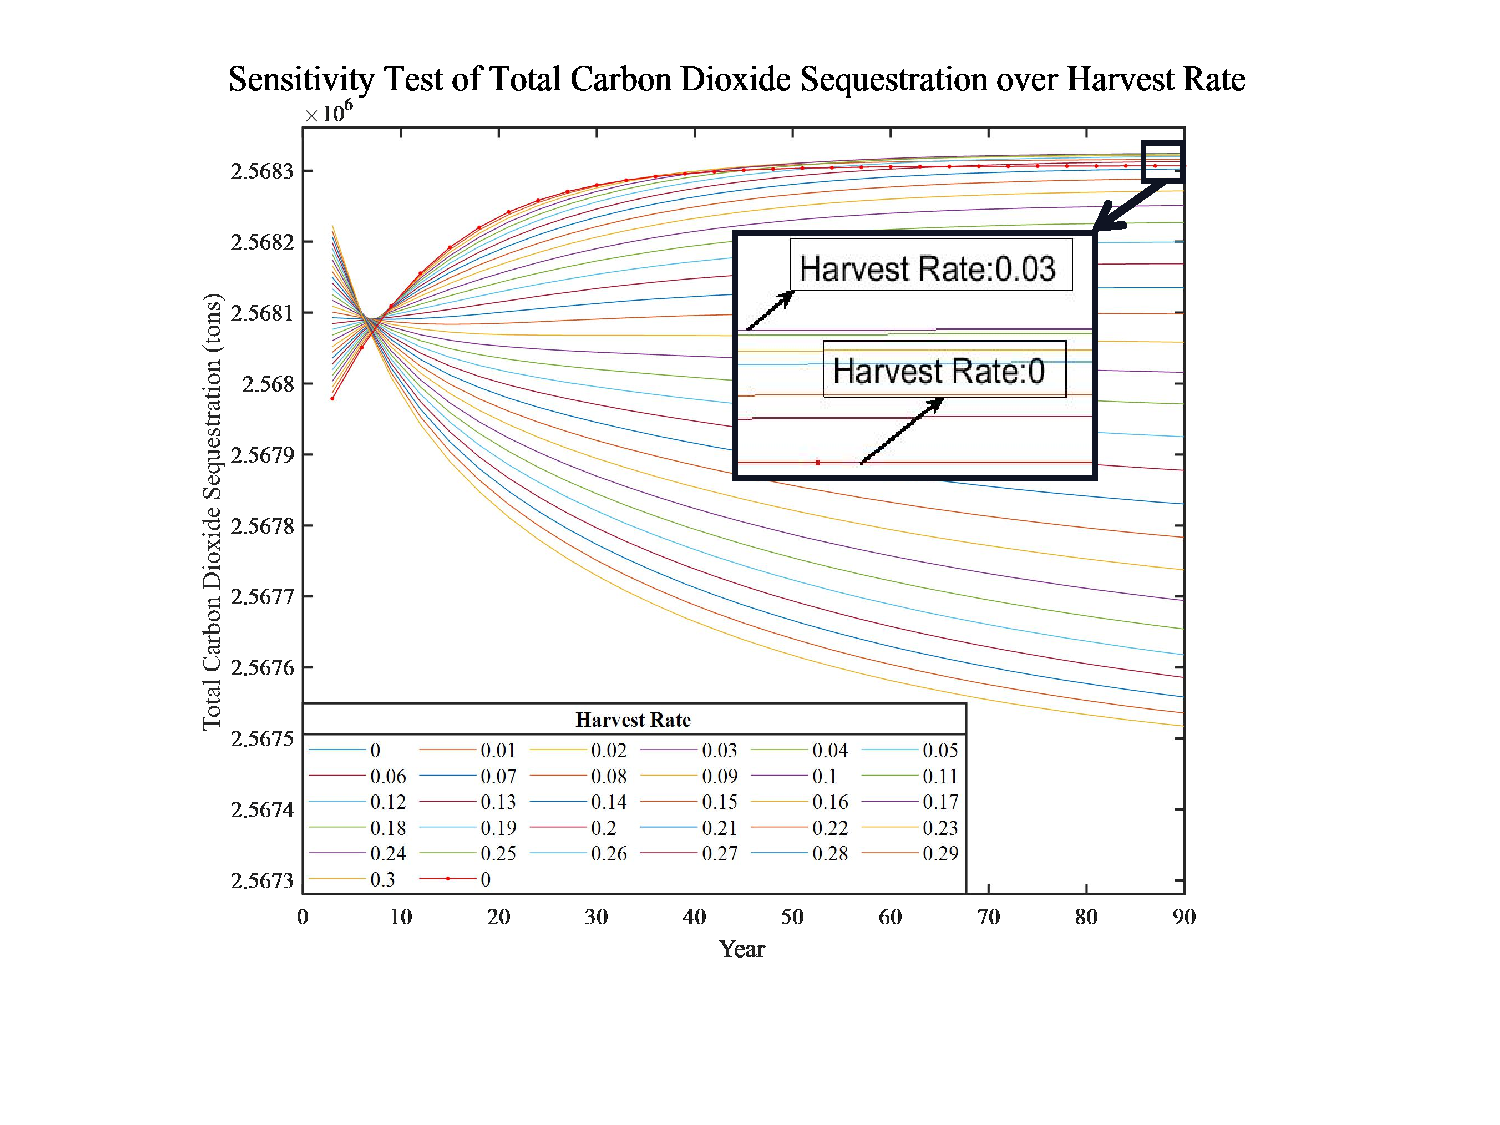
\includegraphics[width = 0.48\textwidth]{code&pic/采伐率.pdf}\label{Harvest Rate sensTest}
  }
  \subfigure[]{
  \centering
  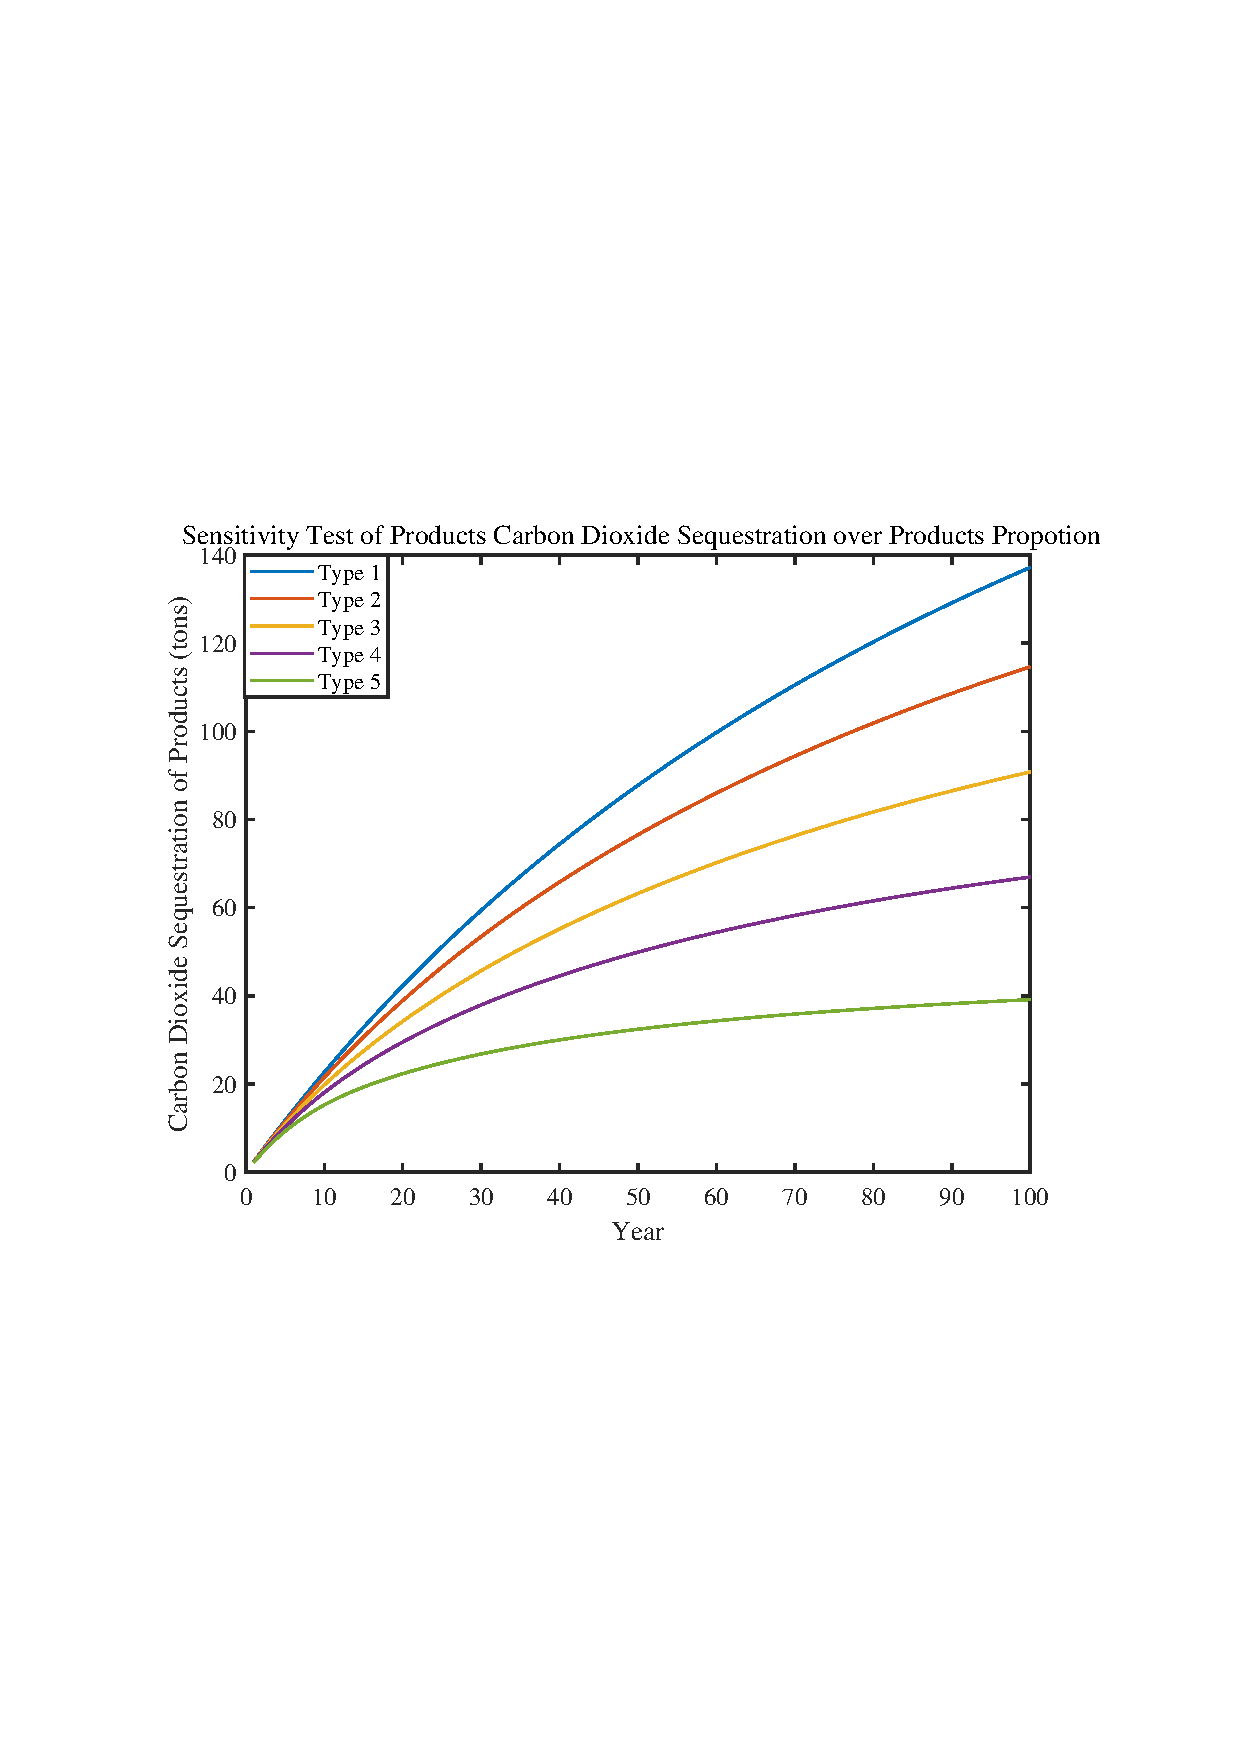
\includegraphics[width = 0.48\textwidth]{code&pic/proportion.pdf}\label{Product Proportion sensTest}
  }

\caption{Results of sensitivity test of Harvest Rate and Product Proportion}
\end{figure}

From what we have discussed above we can draw a very reasonable conclusion that 
there exists an appropriate Harvest Rate, which is 0.03 in our hypothetic Forest, 
that can help the Forest sequester more Carbon Dioxide after 100 years, and
the Forest managers should urge more manufactures of anticorrosive wooden products
rather than those with lower Decomposition Rate. 
\par
What's more, there are some other factors we should take into consideration when 
managing the forests. 


\newpage




\section{Model II}


In order to comprehensively consider the multiple social interests, we add
several indexes which can fully demonstrate the impact of Forests over local 
society. 
\par
The indexes are divided into two aspects, namely \textbf{Carbon Sink} and \textbf{Cultural Value}, and
Carbon Sink weighs 4.123 times than Cultural Value \citep{2007US}. 

\subsection{Carbon Sink}
Figure \ref{CarbonCircle} clearly demonstrates the principle of the carbon circle and roles that Forestry Species play in the 
circle, which helps us to understand the necessary procedure to manage Forestry Carbon Sequestration.

\begin{figure}[htbp]
  \centering
  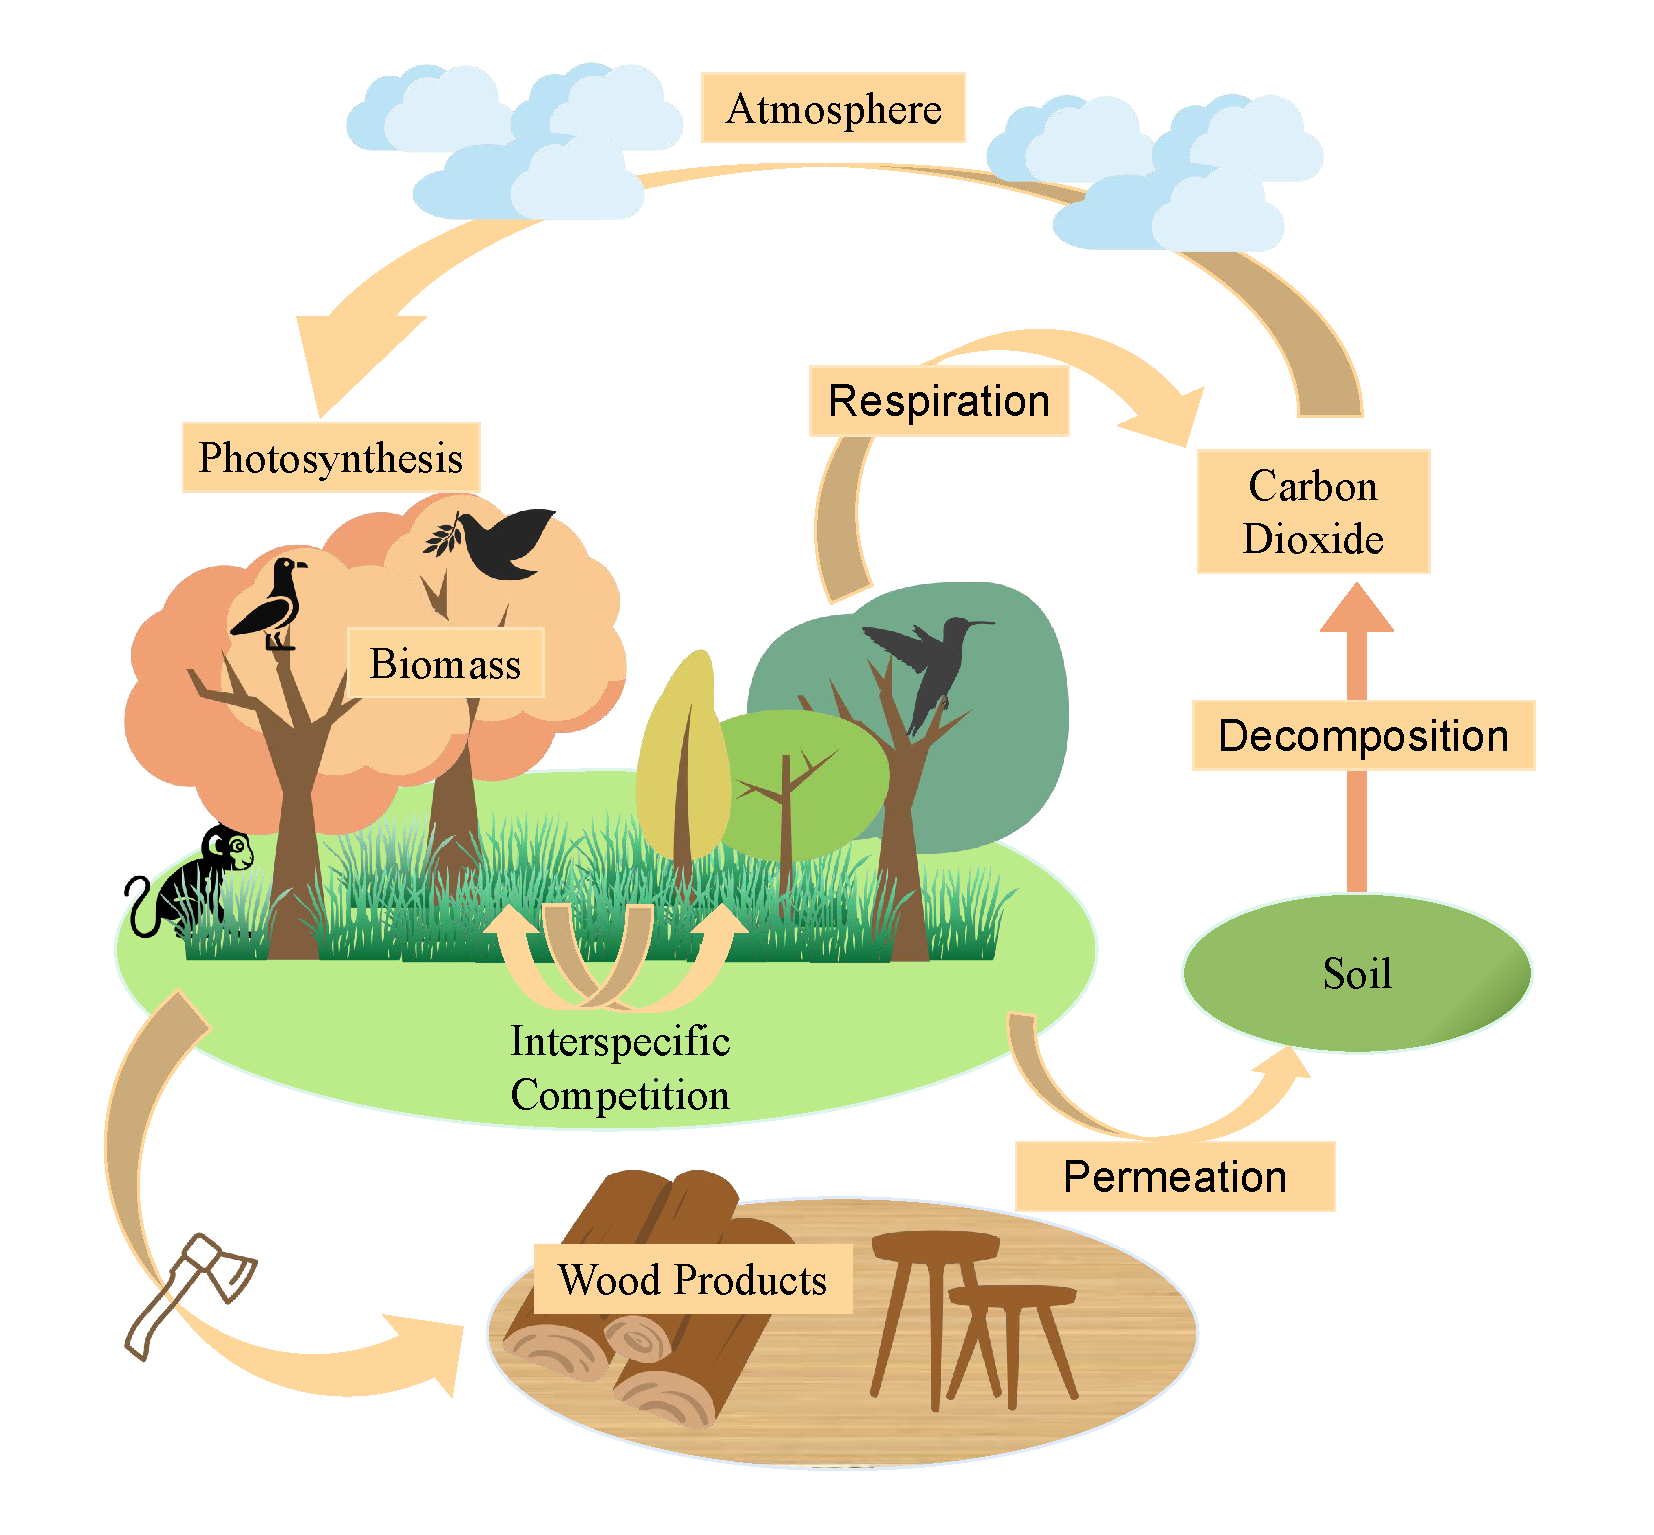
\includegraphics[width = 10cm]{code&pic/大循环.pdf}
  \caption{Carbon Circle in Forest Ecosystem}\label{CarbonCircle}
\end{figure}

Carbon Sink includes the following indexes: \textbf{Carbon Credit Benefit and 
Cost Analysis(CVal), Wooden Product Proportion, Harvest Rate} and \textbf{Interspecific 
Competition}, which will exert influence on carbon sink in this Forest.
\par
CVal is a spreadsheet tool to evaluate the direct benefits and costs of Carbon 
Sequestration contracts for managed forests developed by E.M. (Ted) Bilek,
Peter Becker and Tim McAbee. By inputting a series of parameters of the Forests
such as tract size, $ \rm{CO_2} $ sequestration rate and Carbon price, CVal will
automatically come up with Average cost of trading, Net trading benefit, 
Internal Rate of Return and other important economic indexes. 
\par
Wooden Product Proportion and Harvest Rate are fully discussed above, which will not
be repeated again.
\par
Interspecific Competition is calculated by \textbf{Lotka-Volterra Model}, which is 
used to describe ecology evolution.
Suppose there are two species competing for surviving spaces, namely
Douglas Fir and Pinus Densiflora, whose population sizes are $ N_1 $ and $ N_2 $, population growth rates
are $ r_1 $ and $ r_2 $, carrying capacity $ K_1 $ and $ K_2 $ and coefficients of competition over each other 
are $ \alpha $ and $ \beta $. 
Thus, based on the Logistic growth model, the population of Douglas Fir
can be described as 
$$
  \frac{dN_1}{dt} = r_1\cdot N_1\cdot (\frac{K_1-N_1-\alpha N_2}{K_1})
$$ 
, in which $ \alpha $ is defined as a coefficients of competition of Douglas Fir over Pinus Densiflora,
representing that each Pinus Densiflora will occupy the surviving spaces of
 $ \alpha $ Douglas Firs.
 Similarly, the population of Pinus Densiflora can be described as $$
 \frac{dN_2}{dt} = r_2\cdot N_2\cdot (\frac{K_2-N_2-\beta N_1}{K_2})
 $$ 
Thus, there are four possible results for these two kinds of trees.
\begin{enumerate}
  \item [(1)] Douglas Fir wins, and Pinus Densiflora gets sidelined;
  \item [(2)] Pinus Densiflora wins, and Douglas Fir gets sidelined;
  \item [(3)] Douglas Fir and Pinus Densiflora coexist stably;
  \item [(4)] Douglas Fir and Pinus Densiflora coexist erratically.
\end{enumerate}

Whichever wins, the intensity of intraspecific competition will decline while the
intensity of interspecific competition will roar. If both species suffer high level of
intraspecific competition as well as low interspecific competition, they will stably
coexist, otherwise it leads to unstable coexistence. 
\par
Lotka-Volterra Model can be improved as follows. Suppose a second-order system can be described as the ODE below:
$$
  \frac{d^2x}{dt^2}+a_1(x,\frac{dx}{dt})\frac{dx}{dt} + a_0(x,\frac{dx}{dt})x = 0, \quad \ddot{x} = f(x,\dot{x})
$$  
Suppose $ x = x_1, \frac{dx}{dt} = x_2 $, then
$$
  \frac{dx_2}{dx_1} = \frac{f(x_1,x_2)}{x_2}
$$ 
$$
\begin{cases}
        \frac{dx_1}{dt} = x_2\\
      \frac{dx_2}{dt} =f(x_1,x_2)\\
\end{cases}
$$ 
Suppose $ x_1(t) $ denotes the position of a mass point and $ x_2(t) $ denotes the velocity of the mass point, then the 
solution of the equations depicts the movement of a point in a 2-dimension plane, and the figure of the solution is called
\textbf{Phase Diagram} in physics.
\par
Apply what we discuss above over the previous equations we can draw the improved Model:
$$
  \begin{cases}
    \frac{dr}{dt} = 2(1-\frac{r}{R})-\lambda rf, r(0) = r_0\\
    \frac{df}{dt} = -f + \lambda rf, f(0) = f_0
  \end{cases}
$$ 
\par
Result of the competition between Douglas Fir and Pinus Densiflora is shown in 
Figure \ref{Douglas Fir and Pinus Densiflora result}, while the thermodynamic diagram
of competition intensity between these two species can be seen in Figure \ref{Matrix Douglas Fir and Pinus Densiflora}.

\begin{figure}[htbp]
  \centering
  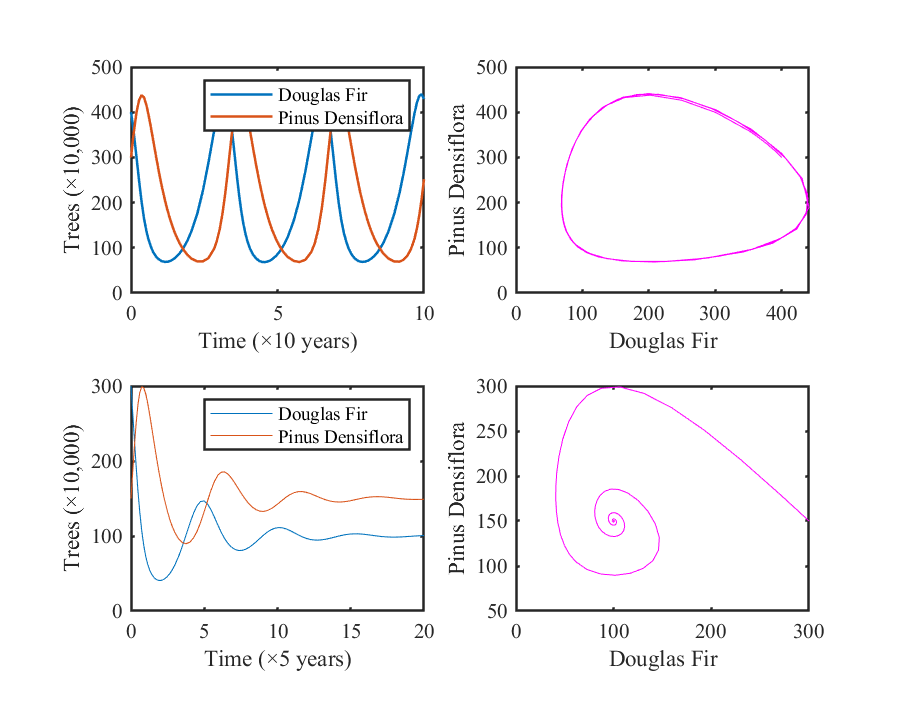
\includegraphics[width = 14cm]{code&pic/Interspecies.eps}
  \caption{Interspecific Competition Result of Douglas Fir and Pinus Densiflora}\label{Douglas Fir and Pinus Densiflora result}
\end{figure}

\begin{figure}[htbp]
  \centering
  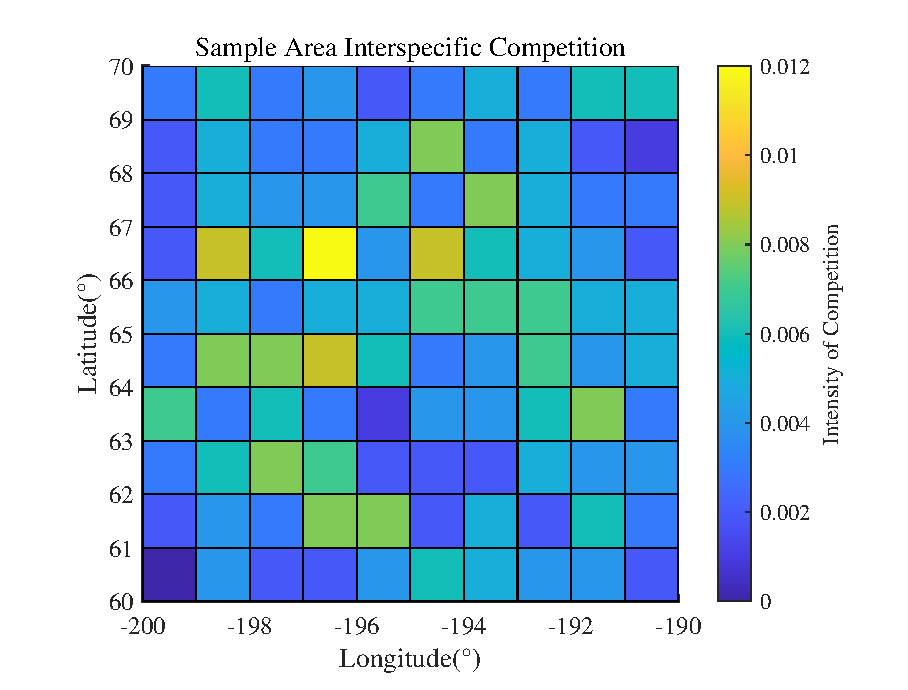
\includegraphics[width = 9cm]{code&pic/Interspecies-matrix.eps}
  \caption{Thermodynamic Diagram of Competition}\label{Matrix Douglas Fir and Pinus Densiflora}
\end{figure}

\subsection{Cultural Value}

\par
In order to further demonstrate the relationship between the five indexes and 
Cultural Value, we abstract three concepts, namely Biodiversity, Development of 
Forest and Forest Influence, from the indexes. The structure of indexes related to 
Cultural Value can be clearly drawn from Figure \ref{Index_CulVal}, 
in which Proportion of Forest and Size
of Forest signify the population the Forest can influence, and Volume of Deadwood
,"an element of biodiversity and, to some extent, an indicator of forest 
management sustainability that deserves to be taken into account in inventories,
especially at the national level"\citep{rondeux2010review}, along with the 
Forest Hierarchy, which provides arboreal 
animals with more habitats, determines the Biodiversity of the Forest.
The Volume of Deadwood of the same type of forest at a similar latitude shares a similar 
constant \citep{2007US}. Size and Proportion of Forest can be searched and estimated on 
map websites, while the Forest Hierarchy is easy to search. 
\begin{figure}[htbp]
  \centering
  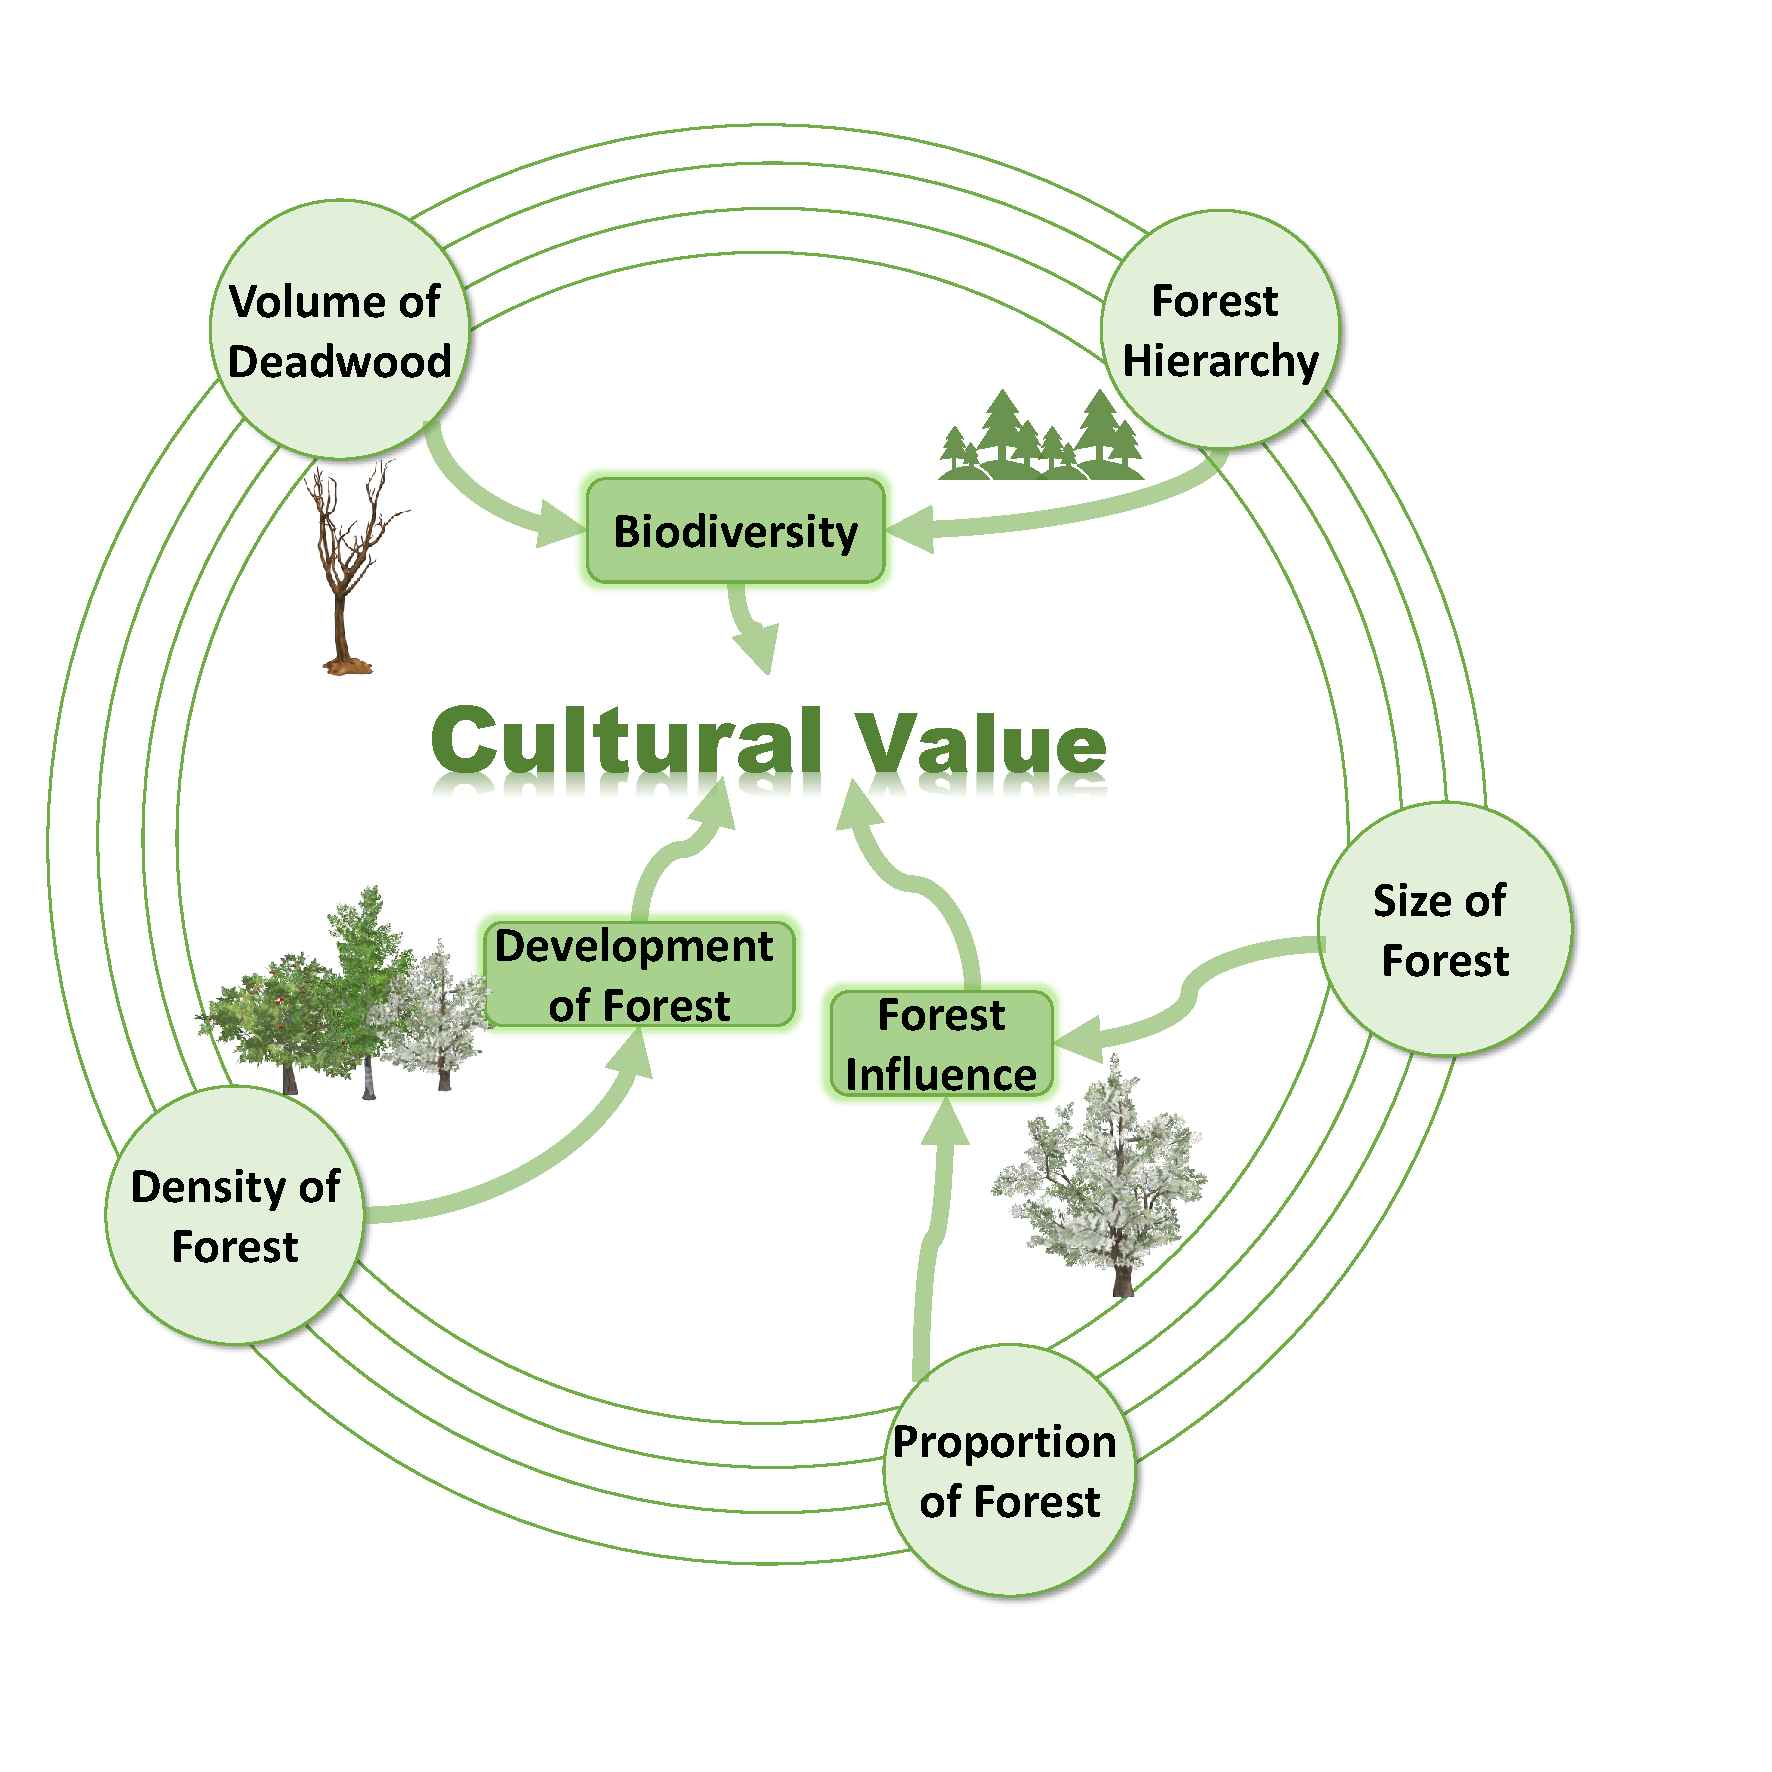
\includegraphics[width = 8cm]{code&pic/Model2.pdf}
  \caption{Influencing indexes of Forest Culture Value}\label{Index_CulVal}
\end{figure}

\subsection{Result and Discussion}

According to Forestry region distribution of the United States in Figure \ref{USmap}, 
we choose four typical kinds of Forests to test our evaluation model, which are
Theropencedrymion, Subboreal coniferous forest, Subtropical 
evergreen broad-leaved forest and Boreal forest. We search and calculate the index values
of these four typical Forests, and come up with their ultimate score by the method below.

\begin{figure}[htbp]
  \centering
  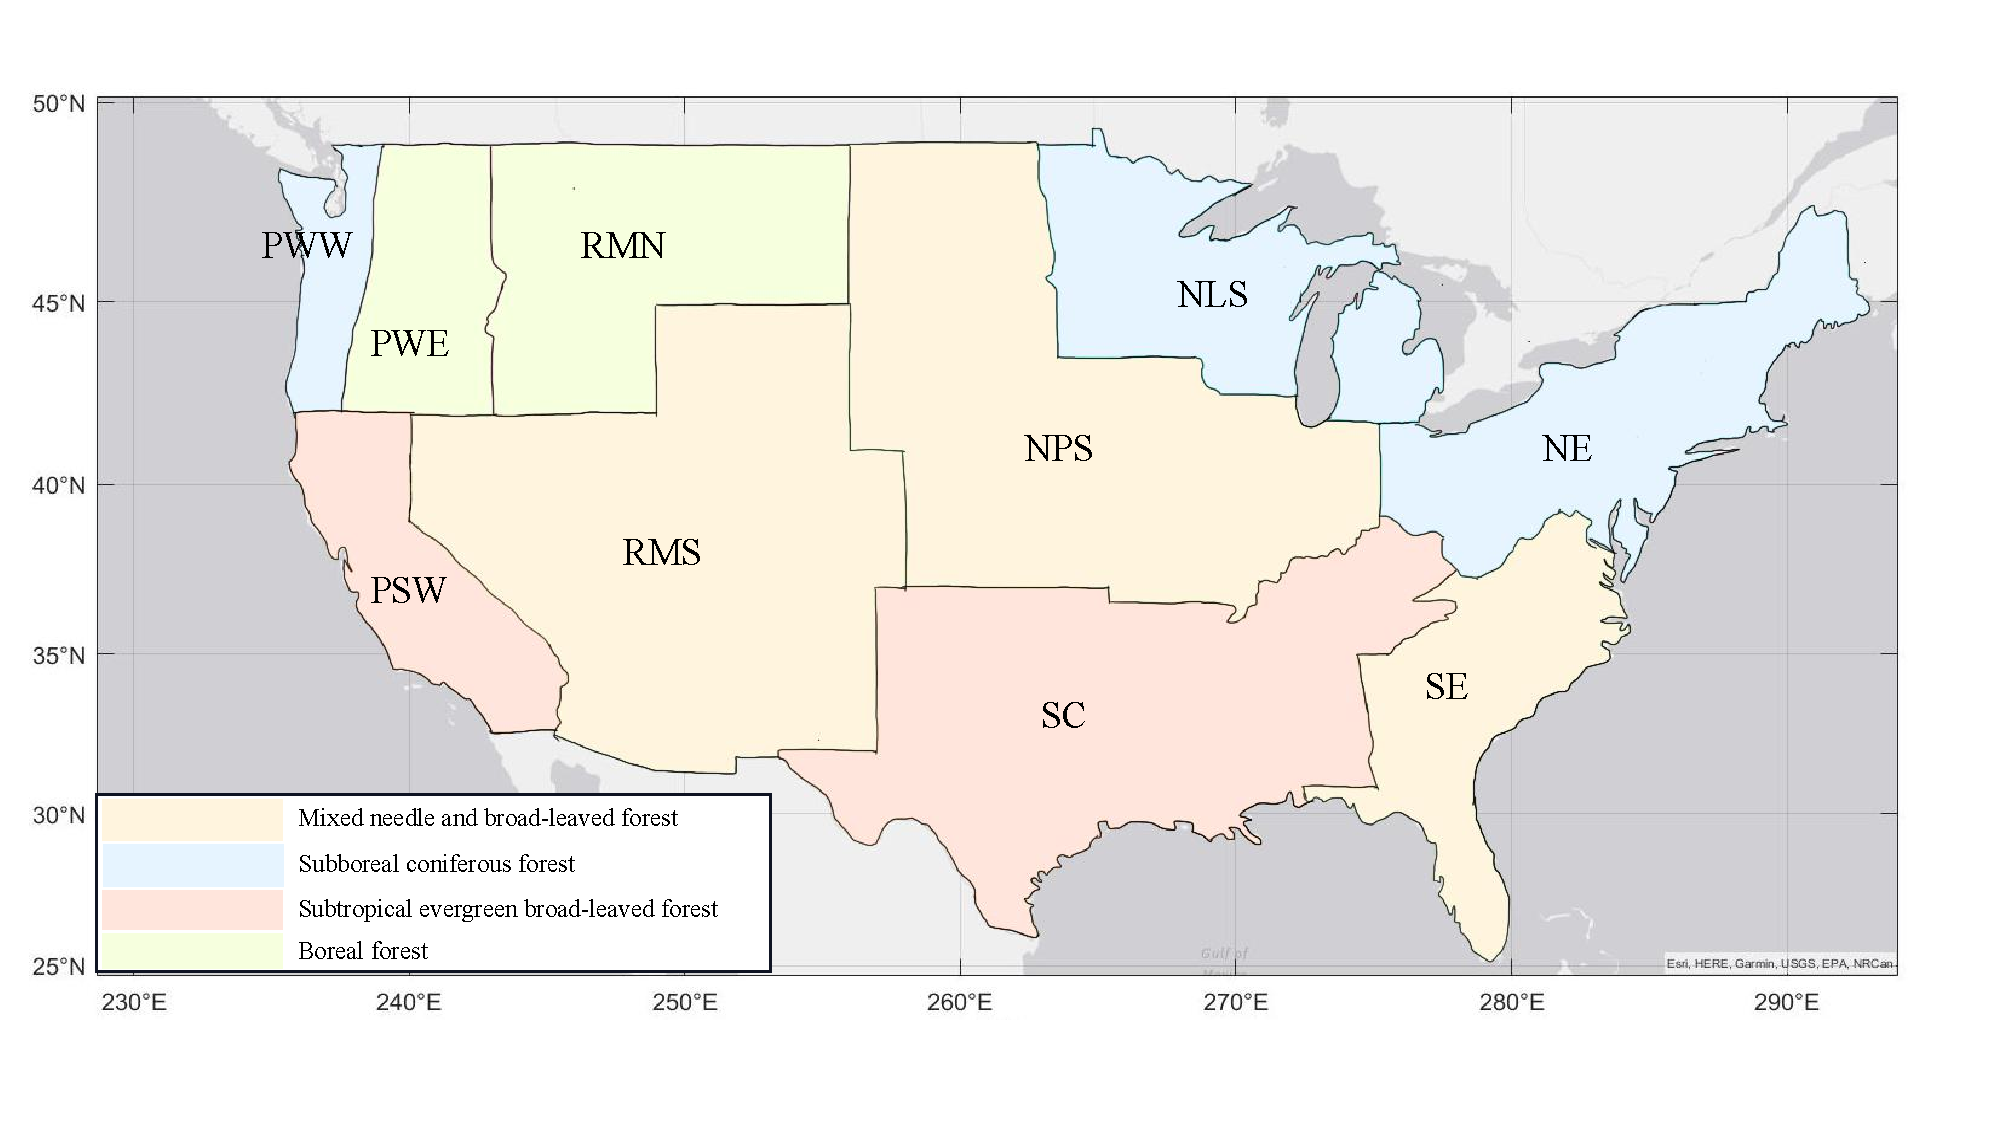
\includegraphics[width = 14cm]{code&pic/美国地图.pdf}
  \caption{Forest division in the United States}\label{USmap}
\end{figure}

\begin{figure}[ht]

  \hfill
  \begin{minipage}[htbp]{0.47\linewidth}
    \begin{flushleft}
      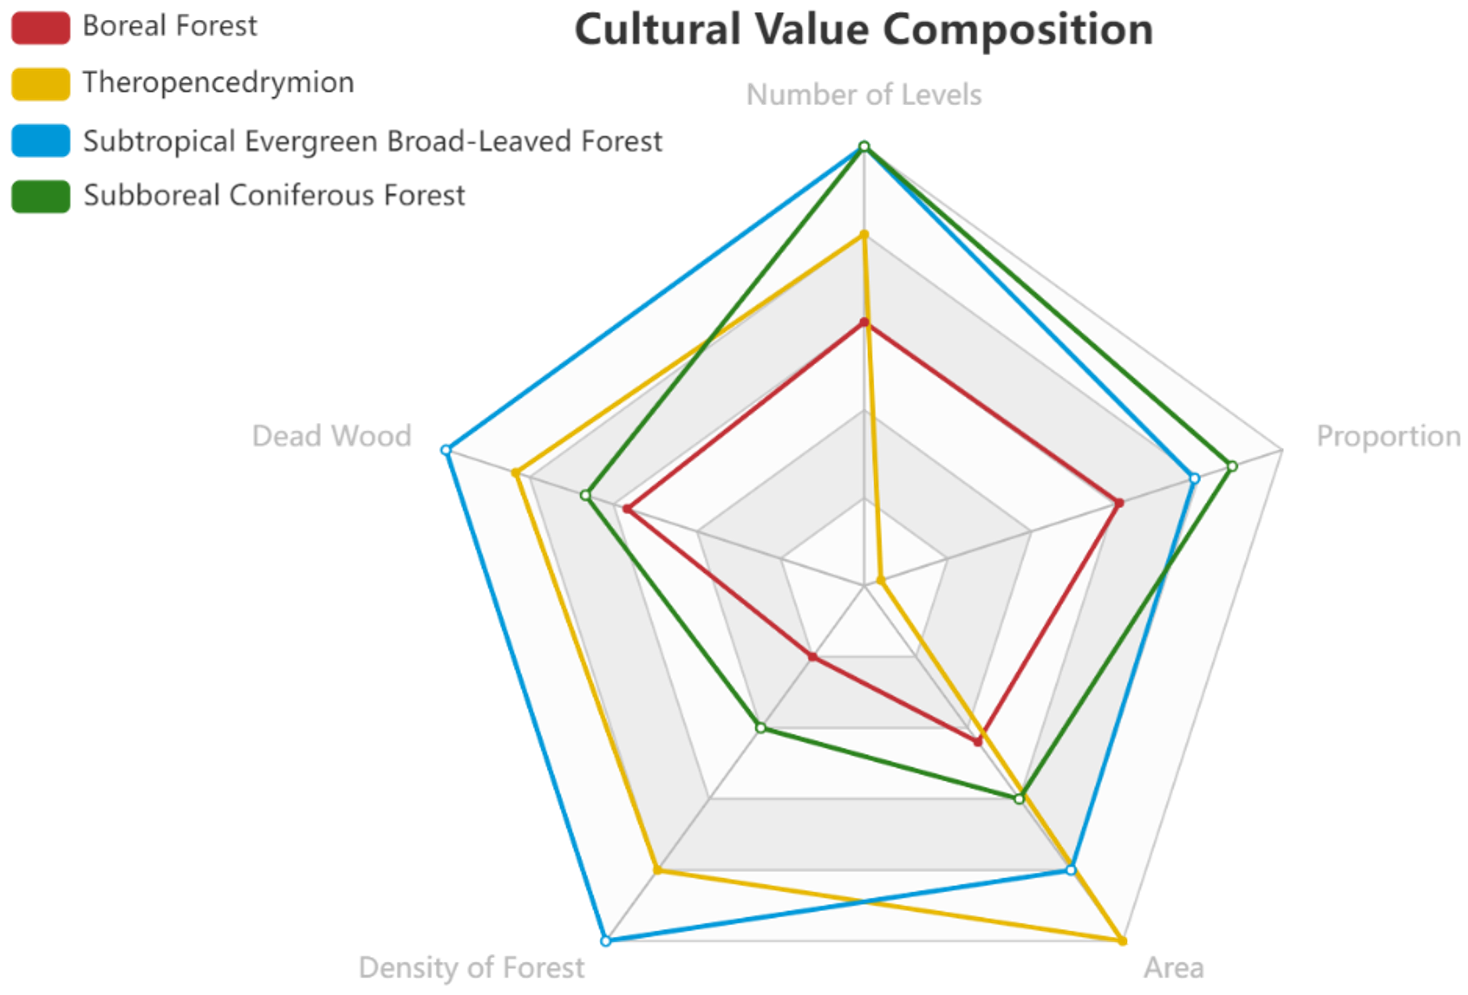
\includegraphics[width = 8cm]{code&pic/Cultural Value Composition.png}
      \caption{Radar Map of Cultural Value}\label{Radar}
    \end{flushleft}
  \end{minipage}
    \begin{minipage}[htbp]{0.45\linewidth}
      The indexes of Carbon Sink are \textbf{Z-score Standardaized} and weighted summed, representing
      Carbon Sink score of this kind of Forest. The indexes of Culture Value are 
      measured by \textbf{Technique for Order Preference by Similarity to an Ideal Solution (TOPSIS)}, 
      whose basic principle is to sort the indexes by detecting the distance between the 
      evaluation object and the worst solution of the optimal solution.  
      If the evaluation object is closest to the optimal solution and furthest 
      away from the worst solution, it is the best. Otherwise, it is not optimal 
      in which all index values of the optimal solution reach the optimal value 
      of all evaluation indexes and all index values of the worst solution reach 
      the worst value of all evaluation indexes. The composition of Cultural Value
      is shown in Figure \ref{Radar}.
  \end{minipage}
\end{figure}


\par
Then the scores of Carbon Sink and Cultural Value are weighted added: 
$$
  \rm{TotalScore} = 4.123\times \rm{CarbonSink} + \rm{Cultural Value}
$$ 
The final scores are shown in Table \ref{ForestScore}, in which we can see that the 
Subtropical Evergreen Broad-leaved Forest ranks the highest concerning the indexes above.
There are some other interesting findings in this table. For instance, both
Theropencedrymion and Subboreal coniferous Forest approach high score in Carbon Sink while 
their Cultural Values are relatively low. However, Boreal Forests are of great
significance in Cultural Value, but it doesn't help much on creating Carbon Sink. 


\begin{table}[htpb!]
  \centering
  \caption{Scores of Four typical Forests} \label{ForestScore}
  \begin{tabular}{m{5.5cm}<{\centering}|m{3cm}<{\centering}|m{3cm}<{\centering}|m{3cm}<{\centering}}
  \rowcolor{lightBlue}  \textbf{Types of Forests}&\textbf{Total Score}&\textbf{Carbon Sink}&\textbf{Cultural Value}\\ \hline
  \rowcolor{white} \textbf{Boreal Forest} & 0.58902 & 0.535529 & 0.809565 \\
  \rowcolor{lightBlue} \textbf{Theropencedrymion} &0.832925&0.892329&0.588001 \\
  \rowcolor{white} \textbf{Subtropical Evergreen Broad-leaved Forest} & 0.993638&0.992332 & 0.999022\\
  \rowcolor{lightBlue} \textbf{Subboreal coniferous Forest} & 0.863477 & 0.932925 &0.577142 \\
  \end{tabular}
\end{table}

In order to figure out the conditions when Harvest Rate is 0 is recommended, 
we calculated the final scores of the four Typical Forests again without Harvest, which 
is shown in Table \ref{ForestScore-NoHarvest}. In comparison with Table \ref{ForestScore}, 
it's obvious that the all the three scores of Boreal Forest, Theropencedrymion and 
Subboreal coniferous Forest increase without harvest, which suggests that 


\begin{table}[htpb!]
  \centering
  \caption{Scores of Four typical Forests without Harvest} \label{ForestScore-NoHarvest}
  \begin{tabular}{m{5.5cm}<{\centering}|m{3cm}<{\centering}|m{3cm}<{\centering}|m{3cm}<{\centering}}
  \rowcolor{lightBlue}  \textbf{Types of Forests}&\textbf{Total Score}&\textbf{Carbon Sink}&\textbf{Cultural Value}\\ \hline
  \rowcolor{white} \textbf{Boreal Forest} & 0.704714 & 0.678393 & 0.813238 \\
  \rowcolor{lightBlue} \textbf{Theropencedrymion} &0.846885&0.908237&0.593933 \\
  \rowcolor{white} \textbf{Subtropical Evergreen Broad-leaved Forest} & 0.98369&0.986493 & 0.972135\\
  \rowcolor{lightBlue} \textbf{Subboreal coniferous Forest} & 0.917332 & 0.947289 &0.79382 \\
  \end{tabular}
\end{table}








\section{Application}
We apply ARIMA model in order to predict the size of Finless Porpoise population in five ex-situ 
conservation areas after 20 years, whose \textbf{algorithm block diagram} 
is shown as Figure \ref{ARIMA_ALGO}.
\par
Under regular circumstances, the time series we obtain in the real world
  has tendency, seasonality and non-stationarity. Thus, it's vital for 
  us to transfer the non-stationary time series to stationary time series
\par
\begin{figure}[ht]
\begin{minipage}[htbp]{0.35\linewidth}
  and make an assumption that the time series is an Auto 
  Regressive Moving Average(ARMA) series to predict the 
  future data. ARMA series is defined as follows.
  \begin{align*}
    &X_t-\phi_1X_{t-1}-\cdots -\phi_pX_{t-p} \\
    &= \epsilon_t - \theta_1\epsilon_{t-1}-\cdots-\theta_q\epsilon_{t-q}
  \end{align*}
 
$ \epsilon_1 $ is a stationary white noise whose average is zero and
deviation is $ \sigma_\epsilon^2 $;$ X_t $is an ARMA series with $ p $ and $ q $
degree, recorded briefly as $ \mathbf{ARMA}(p,q) $ series.
Akaike Information Criterion(AIC) is one of the most commonly used
criterion to determine the degree of $ \mathbf{ARMA}(p,q) $: choose 
$ p,q $ such that 
\begin{equation}\label{AIC}
  \begin{aligned}
    \min \mathbf{AIC} &= n\ln \hat{\sigma_\epsilon^2} \\
    &+ 2(p+q+1)
  \end{aligned}
\end{equation}
$ n $ is the capacity of sample;$ \hat{\sigma_\epsilon^2} $ is the
estimation of $ \sigma_\epsilon^2 $ relating to $ p $ and $ q $.
Suppose $ p = \hat{p}, q = \hat{q} $, such that equation(\ref{AIC}) reaches the minimum,
than we deem the series is $ \mathbf{ARMA}(\hat{p},\hat{q}) $. 
\end{minipage}
\hfill
\begin{minipage}[htbp]{0.55\linewidth}
  \begin{flushleft}
    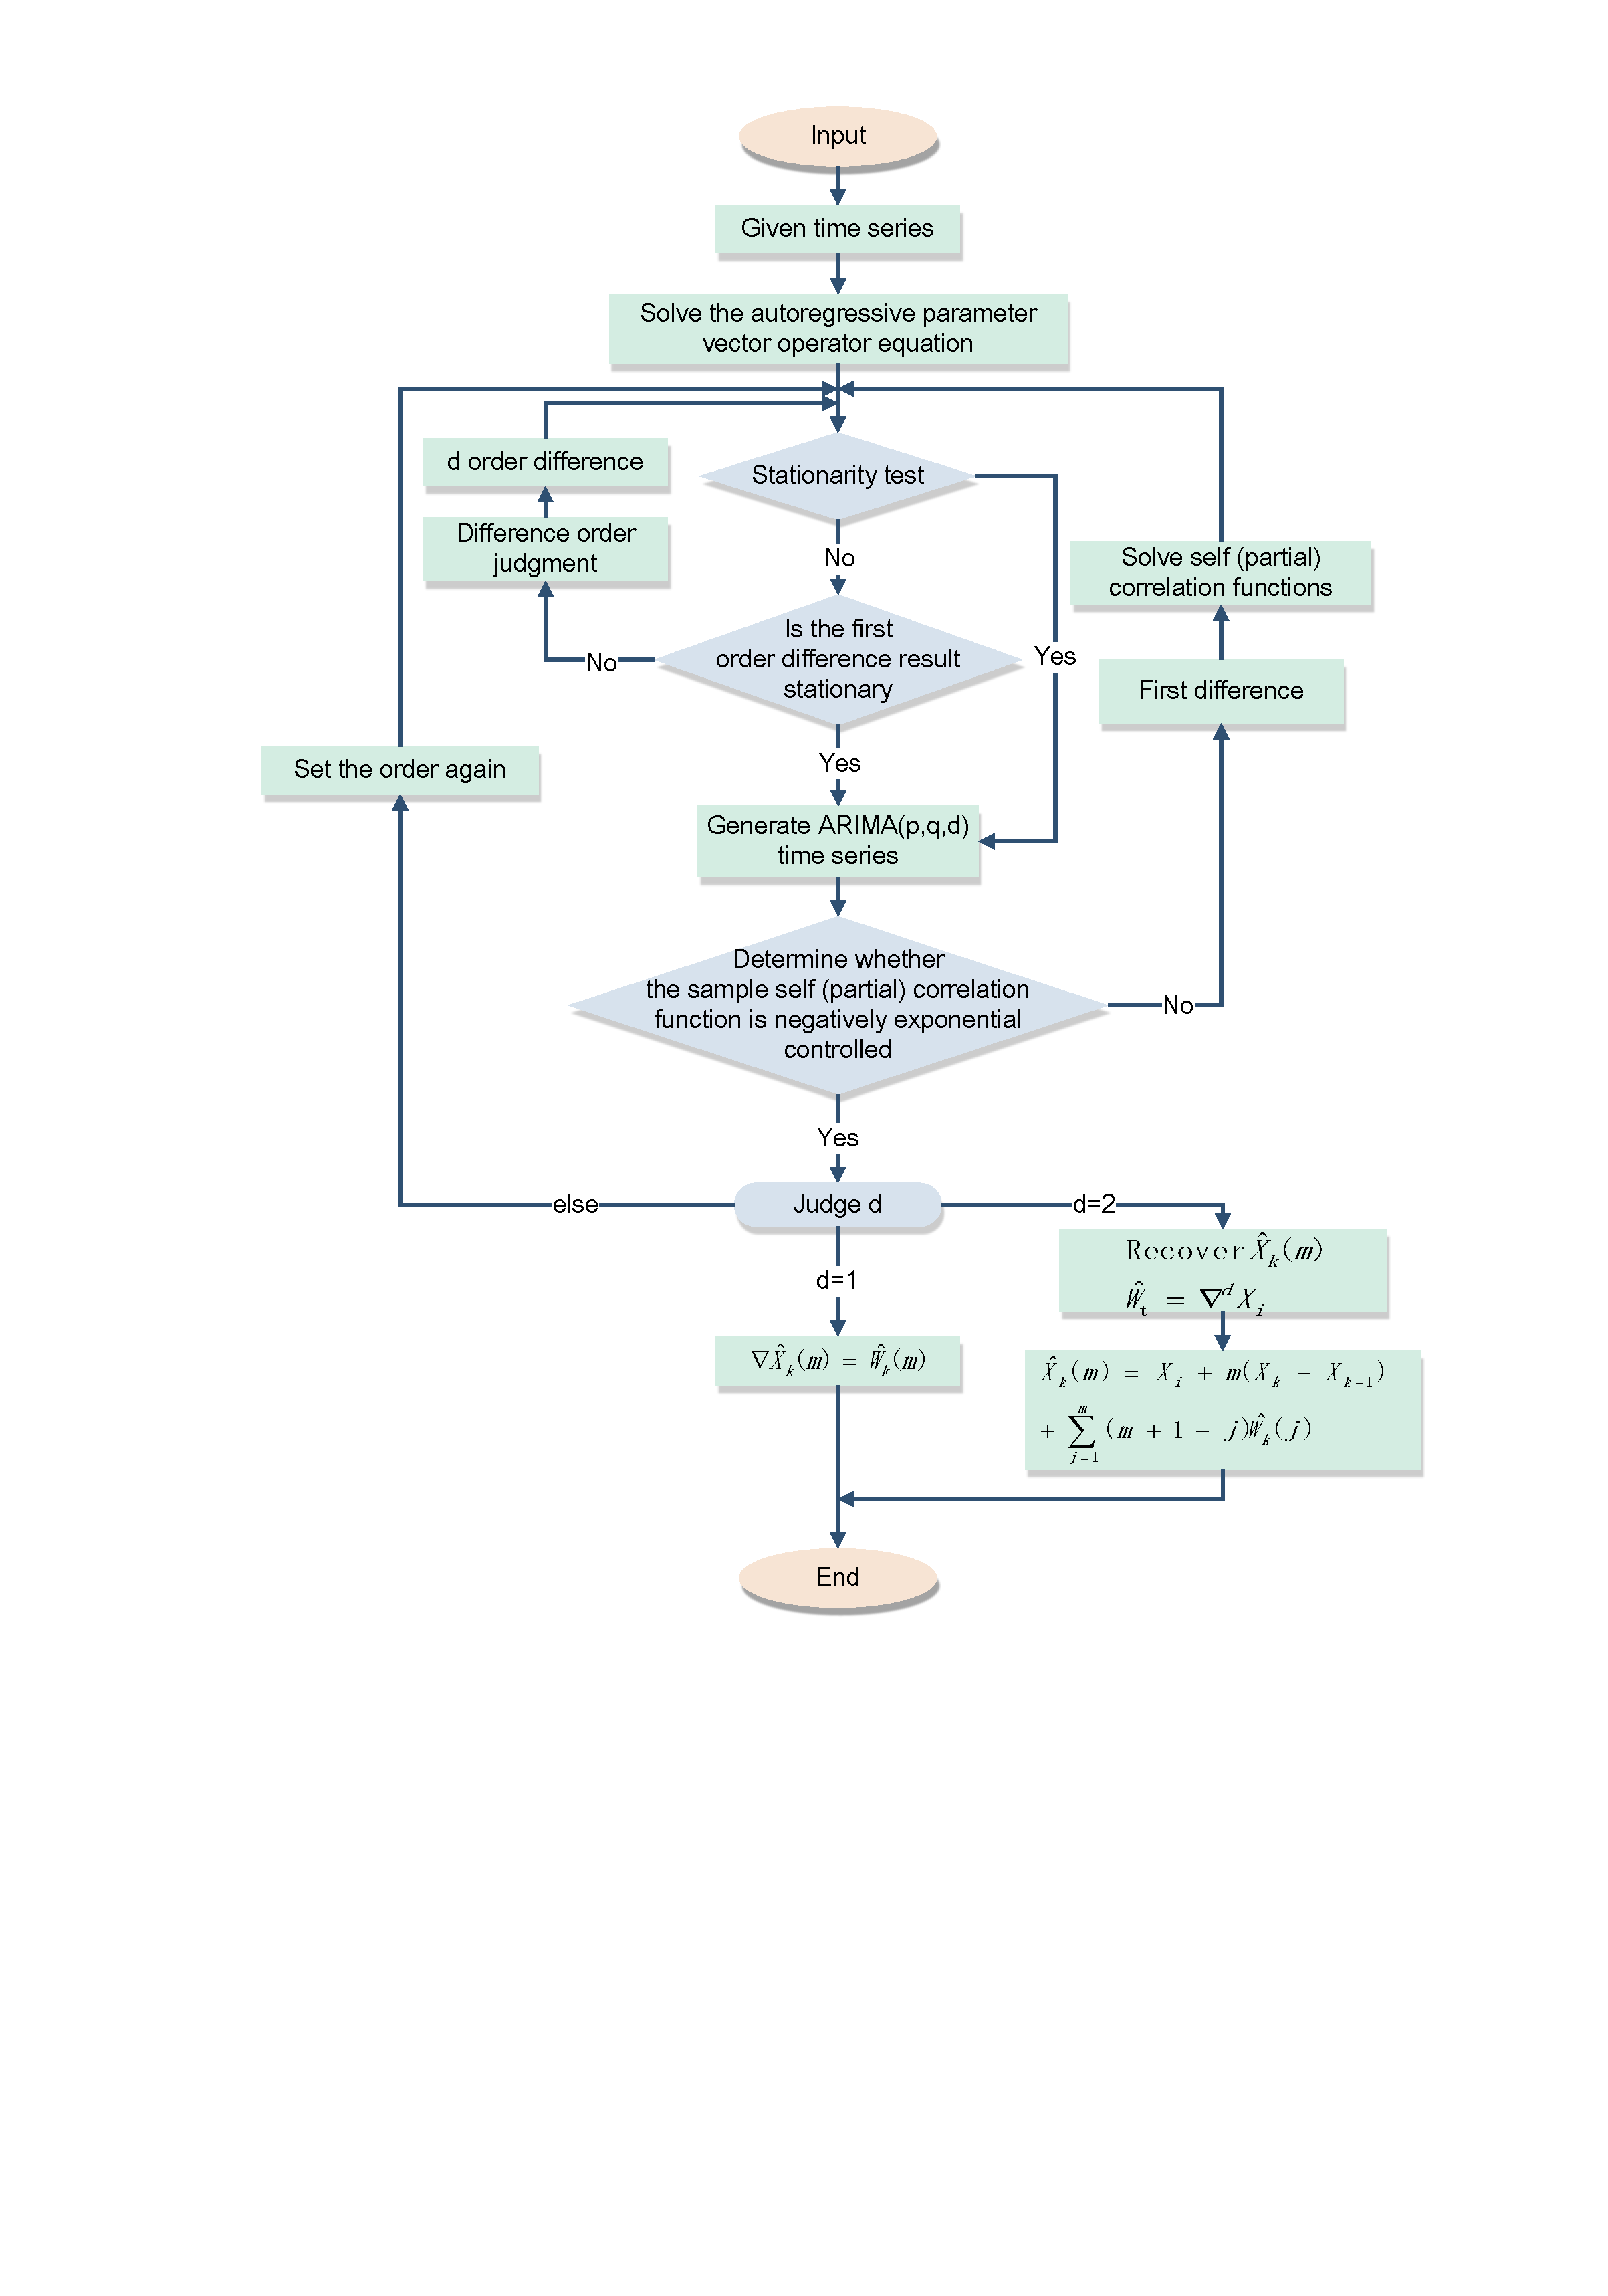
\includegraphics[width =11cm]{code&pic/ARIMA_裁剪页面.pdf}
   \caption{Algorithm Block of ARIMA}\label{ARIMA_ALGO}
  \end{flushleft}
\end{minipage}
\end{figure}



\par
Suppose $ \mathbf{ARMA}(p,q) $ series has an unknown average parameter $ \mu $,
the model becomes
$$
  \phi(B)(X_y-\mu) = \theta(B)\epsilon_t,
$$   
meanwhile, the number of unknown parameters is $ k = p+q+2 $, the AIC is:
choose $ p,q $ such that
\begin{equation}\label{AIC_unknown}
  \min \mathbf{AIC} = n\ln\hat{\sigma_\epsilon^2}+2(p+q+2).
\end{equation}  
In fact, equations (\ref{AIC}) and (\ref{AIC_unknown}) have the same minimum point $ \hat{p},\hat{q} $.
After that, we usually choose $ p = 1, q = 1 $ to make parameter estimation 
over ARMA model.
\par
It's demonstrated that the differential operation can stabilize 
certain class of non-stationary series. And It's emphasized that 
stationary test must be conducted previously. Stationary test can 
be applied by calculating sample autocorrelation function and 
sample coefficient of partial function. 
\par
If the functions are truncated or trending to 0 (meaning being controlled
by negative index), than the series belongs to ARMA model.
\par
If at least one of the functions above is not truncated or trending to 0, than
it's not stationary.
\par
Suppose the series is non-stationary, which can be transformed to 
a stationary series by $ d $ -degree differential operation, denoted
as $ \mathbf{ARIMA}(p,q,d) $ series,than differentiate the sample by
$ d $ -degree:
$$
  W_t = \nabla^dX_t,\quad t = d+1,\dots , n
$$ 
After that, apply stationary test on $ W_t $ and repeat steps above 
until it becomes a stationary series, Than $ W_t $(which is denoted
as $ X_t $ ) complies ARMA model. 
\par

\begin{figure}
  \centering
  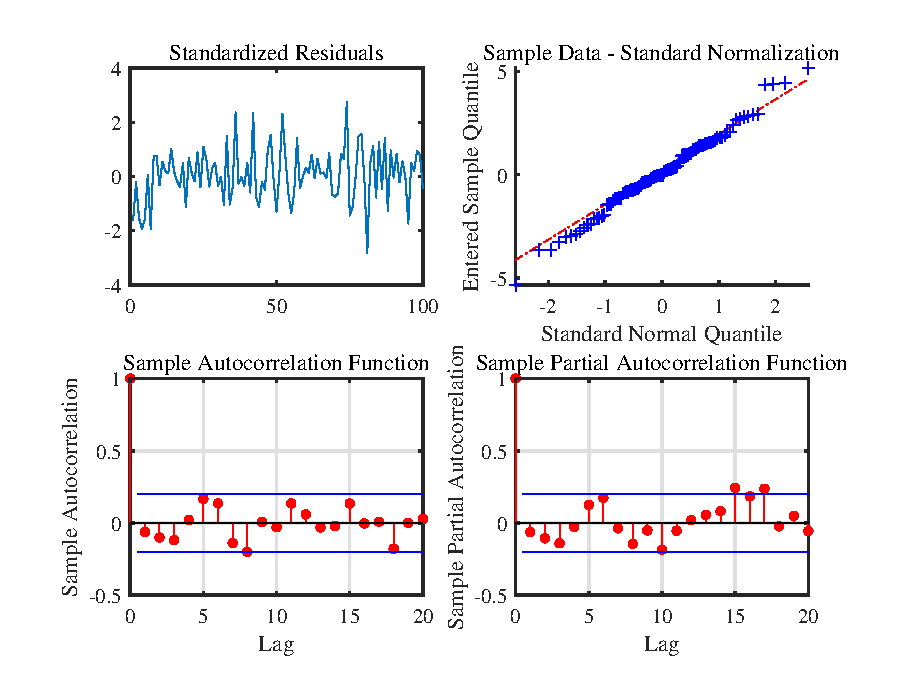
\includegraphics[width = 10cm]{code&pic/ARIMA残差&自相关互相关系数.eps}
\end{figure}



% \begin{figure}[htbp]
%   \centering

%   \subfigure[Sample Autocorrelation Function and Sample Partial Autocorrelation Function]{
%   \centering
%   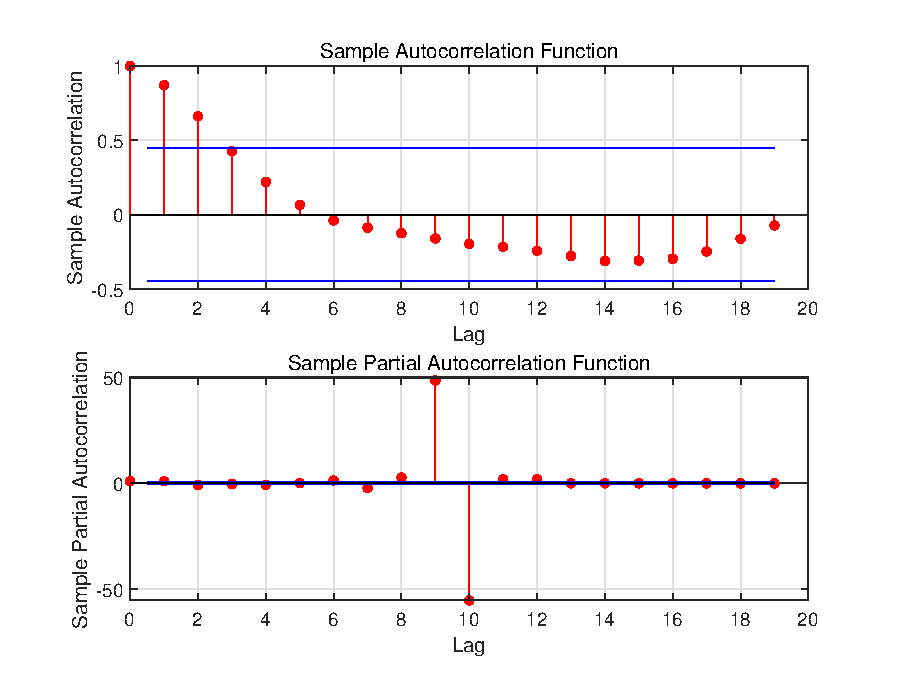
\includegraphics[width = 0.3\textwidth]{codes/1.eps}
%   }
% \quad
%   \subfigure[Sample Autocorrelation Function and Sample Partial Autocorrelation Function]{
%   \centering
%   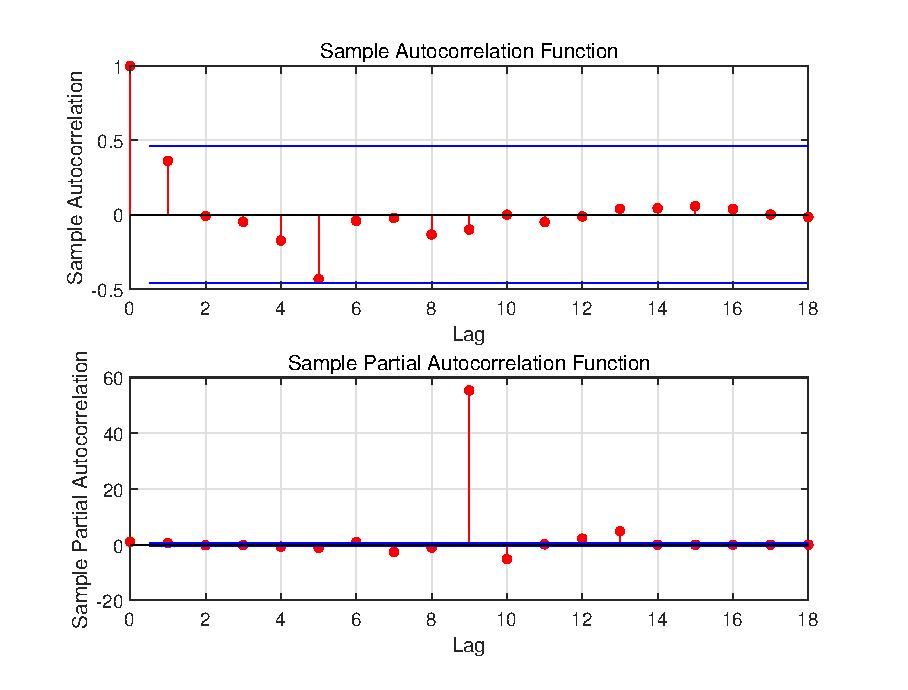
\includegraphics[width = 0.3\textwidth]{codes/3.eps}
%   }
% \par
%   \subfigure[ARIMA Sequence Prediction of Conservation]{
%   \centering
%   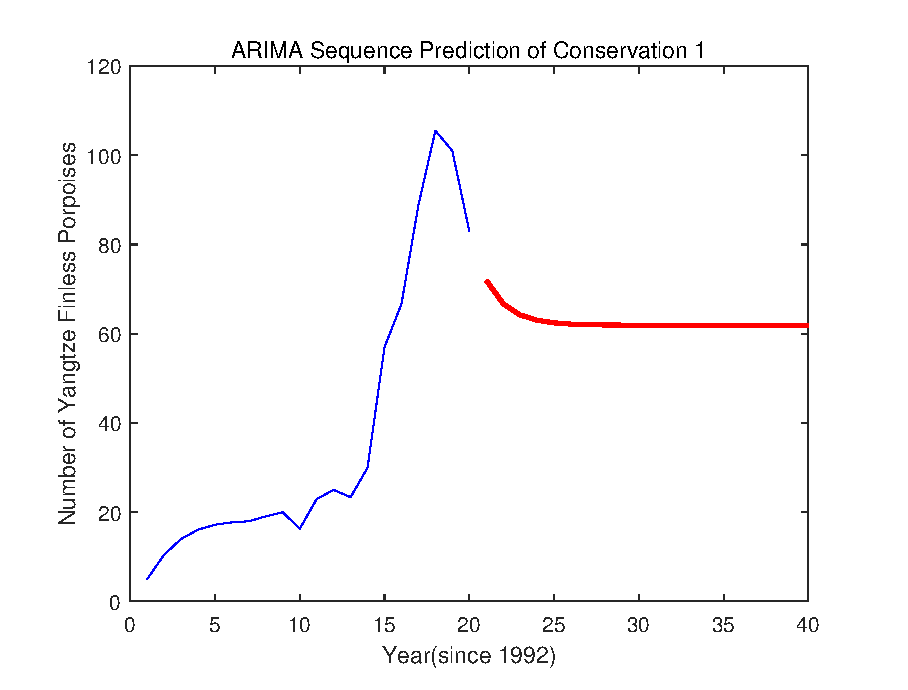
\includegraphics[width = 0.3\textwidth]{codes/2.eps}\label{ARIMA Sequence}
%   }
% \quad
% \subfigure[Standardaized Residuals and QQ figure]{
%   \centering
%   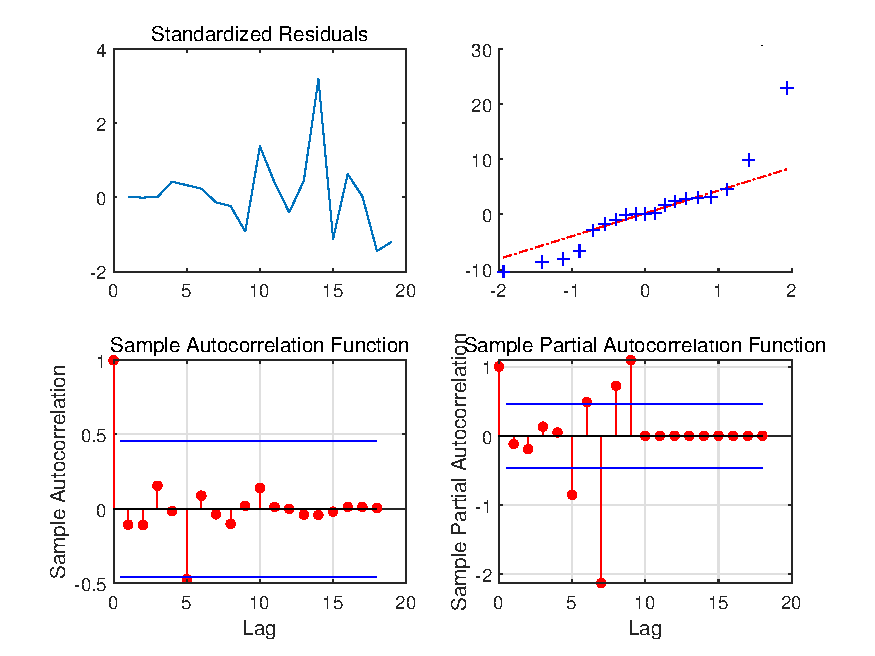
\includegraphics[width =0.3\textwidth]{codes/4.pdf}
% }
% \caption{Results of ARIMA model}
% \end{figure}



















\section{Sensitivity Test}
\begin{figure}[ht]
  \begin{minipage}[htbp]{0.4\linewidth}
    We assume that the density of the forest population follows the Logistic Model,
    and the \textbf{Carrying Capacity of the trees} is $ K $. From the Carbon Sequestration
    probability predicted on the right we can draw a reasonable conclusion that
    the Logistic Model will result into chaos after 3.6 rounds of harvests. 

  \end{minipage}
  \hfill
  \begin{minipage}[htbp]{0.55\linewidth}
    \begin{flushright}
      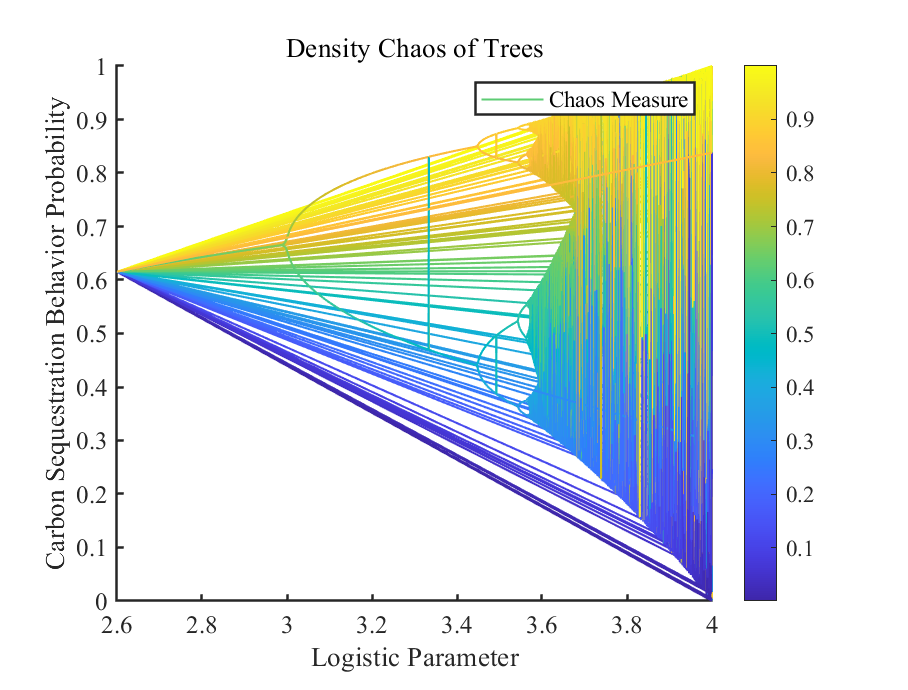
\includegraphics[width = 9cm]{code&pic/Logistic.eps}
    \end{flushright}
  \end{minipage}
\end{figure}
\section{Evaluation of Model}

\textbf{Strength:}


\section{Conclusions}



\newpage
\phantomsection\addcontentsline{toc}{section}{Policy Advice on Finless Porpoise Conservation}\tolerance=500
\memoto{Relavant Authorities}
\memofrom{MCM/ICM team 2215432}
\memodate{\today}

\begin{memo}[Policy Advice on Finless Porpoise Conservation]

  
\end{memo}




\newpage

%这一行是用来将Reference添加到目录的
\phantomsection\addcontentsline{toc}{section}{Refence}\tolerance=500

\bibliographystyle{apacite}
\bibliography{reference.bib}


\lhead{\small\sffamily \team}
% \rhead{\small\sffamily Page \thepage\ }

\begin{appendices}

\textbf{Parameter Settings of hypothetic Forest}

$ a=0.00006303;
D1=0.25;
D2=0.35;
b=1.8218;
H1=25;
H2=10;
c=1.0282;$

$
N1=5000;
N2=5000;
s=0.001;%折损率
$

$
d=[0.125984252 0.031496063 0.251968504 0.503937008 0.062992126 0.015748031 
0.007874016];
 $ 

\begin{figure}[htbp]
  \centering
  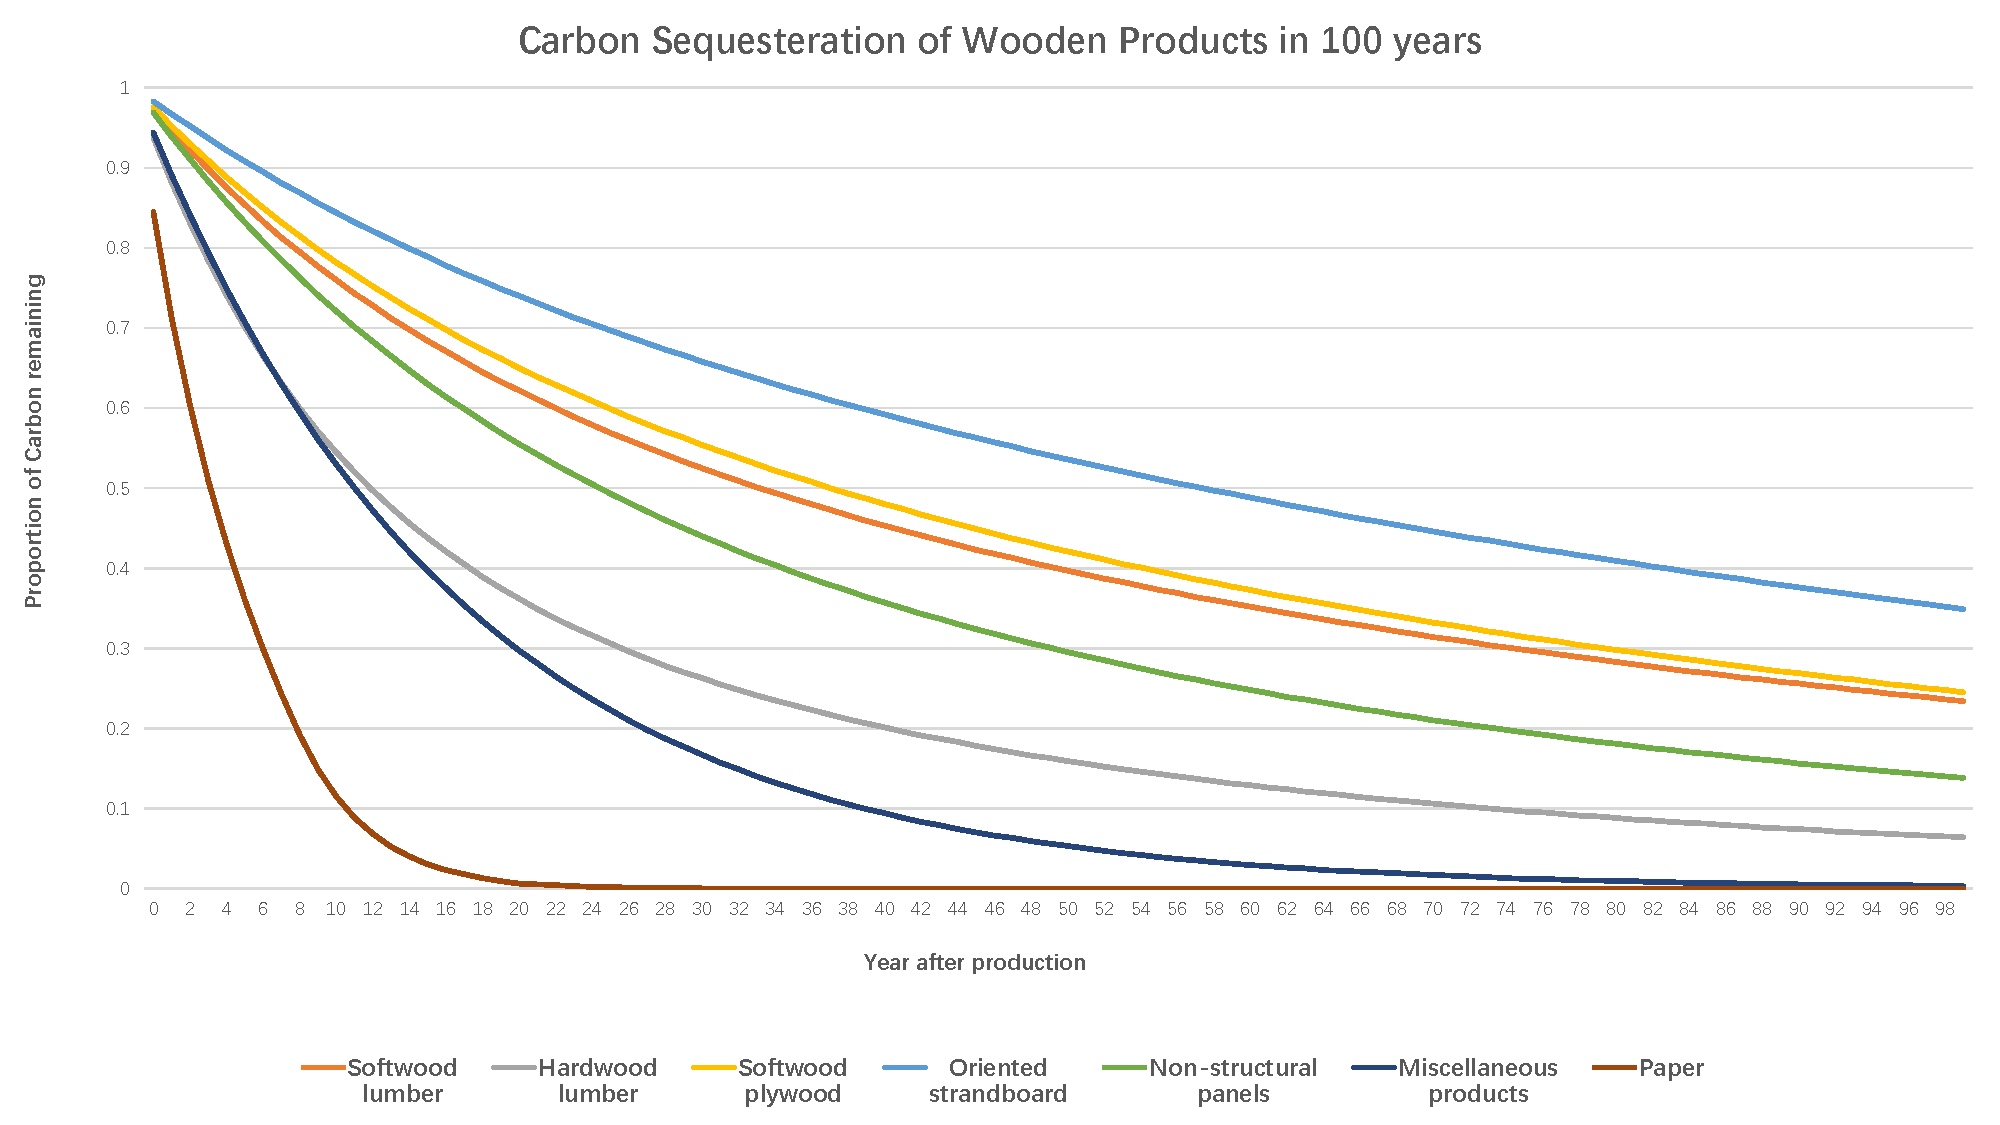
\includegraphics[width = 14cm]{code&pic/产品腐败数据.pdf}
\end{figure}
\begin{table}[htbp]
  \begin{tabular}{c|ccccc}
  \textbf{Types of wooden production}                        & \textbf{Type1} & \textbf{Type2} & \textbf{Type3} & \textbf{Type4} & \textbf{Type5} \\ \hline
  \cellcolor[HTML]{FFFFFF}\textbf{Softwood lumber}      & 0.125984252    & 0.178571429    & 0.142857143    & 0.107142857    & 0.031496063    \\
  \cellcolor[HTML]{FFFFFF}\textbf{Hardwood lumber}      & 0.031496063    & 0.107142857    & 0.142857143    & 0.178571429    & 0.125984252    \\
  \cellcolor[HTML]{FFFFFF}\textbf{Softwood plywood}      & 0.251968504 & 0.214285714 & 0.142857143 & 0.071428571 & 0.015748031 \\
  \cellcolor[HTML]{FFFFFF}\textbf{Oriented strandboard} & 0.503937008    & 0.25           & 0.142857143    & 0.035714286    & 0.007874016    \\
  \cellcolor[HTML]{FFFFFF}\textbf{Non-structural panels} & 0.062992126 & 0.142857143 & 0.142857143 & 0.142857143 & 0.062992126 \\
  \textbf{Miscellaneous products}                       & 0.015748031    & 0.071428571    & 0.142857143    & 0.214285714    & 0.251968504    \\
  \textbf{Paper}                                        & 0.007874016    & 0.035714286    & 0.142857143    & 0.25           & 0.503937008   
  \end{tabular}
  \end{table}
% \textbf{\textcolor[rgb]{0.98,0.00,0.00}{Input python source:}}
% \lstinputlisting[language=python]{./codes/verhulst.py}


% \textbf{\textcolor[rgb]{0.98,0.00,0.00}{Input matlab source:}}
% \lstinputlisting[language=Matlab]{./codes/lagrange_main.m}


\end{appendices}


\end{document}

